%Este trabalho está licenciado sob a Licença Creative Commons Atribuição-CompartilhaIgual 3.0 Não Adaptada. Para ver uma cópia desta licença, visite https://creativecommons.org/licenses/by-sa/3.0/ ou envie uma carta para Creative Commons, PO Box 1866, Mountain View, CA 94042, USA.

%%%%%%%%%%%%%%%%%%%%%%%%%%%%%%%%%%%%%%%%%%
% ATENÇÃO
%
% POR SEGURANÇA, NÃO EDITE ESTE ARQUIVO
%
%%%%%%%%%%%%%%%%%%%%%%%%%%%%%%%%%%%%%%%%%

\documentclass[12pt]{book}

\input preambulo.tex
\setlength{\headheight}{30pt}
\begin{document}

\frontmatter

\title{Cálculo Vetorial\\\small{Um Livro Colaborativo}}
\author{}
\date{\today}
\ifishtml
\else
\addcontentsline{toc}{chapter}{Capa}
\fi

\maketitle

%Este trabalho está licenciado sob a Licença Creative Commons Atribuição-CompartilhaIgual 3.0 Não Adaptada. Para ver uma cópia desta licença, visite https://creativecommons.org/licenses/by-sa/3.0/ ou envie uma carta para Creative Commons, PO Box 1866, Mountain View, CA 94042, USA.

\chapter*{Organizadores}
\addcontentsline{toc}{chapter}{Organizadores}

\begin{itemize}
\item[] Esequia Sauter - UFRGS
\item[] Fabio Souto de Azevedo - UFRGS
\item[] Pedro Henrique de Almeida Konzen - UFRGS
\end{itemize}
%Este trabalho está licenciado sob a Licença Creative Commons Atribuição-CompartilhaIgual 3.0 Não Adaptada. Para ver uma cópia desta licença, visite https://creativecommons.org/licenses/by-sa/3.0/ ou envie uma carta para Creative Commons, PO Box 1866, Mountain View, CA 94042, USA.

\chapter*{Colaboradores}
\addcontentsline{toc}{chapter}{Colaboradores}

Este material é fruto da escrita colaborativa. Veja a lista de colaboradores em:
\begin{center}
  \url{https://github.com/reamat/CalculoNumerico/graphs/contributors}
\end{center}

Para saber mais como participar, visite o site oficial do projeto:
\begin{center}
  \url{https://www.ufrgs.br/reamat/CalculoNumerico}
\end{center}
ou comece agora mesmo visitando nosso repositório GitHub:
\begin{center}
  \url{https://github.com/reamat/CalculoNumerico}
\end{center}


% Aqui você encontra a lista de colaboradores do livro. Esta lista contém somente aqueles que explicitamente se manifestaram a favor de terem seus nomes registrados aqui. A lista completa de colaborações pode ser obtida no repositório GitHub do livro:
% \begin{center}
%   \url{https://github.com/livroscolaborativos/CalculoNumerico}
% \end{center}
% Além das colaborações via GitHub, o livro também recebe colaborações via discussões, sugestões e avisos deixados em nossa lista de e-mails:
% \begin{center}
% \url{livro_colaborativo@googlegroups.com}
% \end{center}
% Estas colaborações não estão listadas aqui, mas podem ser vistas no site do grupo de e-mails.

% Caso encontre algum equívoco ou veja seu nome listado aqui por engano, por favor, entre em contato conosco por e-mail:
% \begin{center}
%   \url{livroscolaborativos@gmail.com}
% \end{center}
% ou via o repositório GitHub.

% \begin{table}[h!]
%   \centering
%   \caption{Lista de colaboradores}
%   \label{tab:colaboradores}
%   \begin{tabular}{llll} \hline
%     Nome & Afiliação & E-Mail & 1ª Contribuição\\ \hline
%     Rafael Sachetto Oliveira & Universidade Federal de São João del-Rei & sachetto@ufsj.edu.br & \#158 \\
%     Debora Lidia Gisch & -x- & -x- & \#63 \\
%     \hline
%   \end{tabular}
% \end{table}

%Este trabalho está licenciado sob a Licença Creative Commons Atribuição-CompartilhaIgual 3.0 Não Adaptada. Para ver uma cópia desta licença, visite https://creativecommons.org/licenses/by-sa/3.0/ ou envie uma carta para Creative Commons, PO Box 1866, Mountain View, CA 94042, USA.

\chapter*{Licença}
\addcontentsline{toc}{chapter}{Licença}

Este trabalho está licenciado sob a Licença Creative Commons Atribuição-CompartilhaIgual 3.0 Não Adaptada. Para ver uma cópia desta licença, visite https://creativecommons.org/licenses/by-sa/3.0/ ou envie uma carta para Creative Commons, PO Box 1866, Mountain View, CA 94042, USA.

%Este trabalho está licenciado sob a Licença Creative Commons Atribuição-CompartilhaIgual 3.0 Não Adaptada. Para ver uma cópia desta licença, visite https://creativecommons.org/licenses/by-sa/3.0/ ou envie uma carta para Creative Commons, PO Box 1866, Mountain View, CA 94042, USA.

\chapter*{Nota dos organizadores}
\addcontentsline{toc}{chapter}{Nota dos organizadores}

Nosso objetivo é de fomentar o desenvolvimento de materiais didáticos pela colaboração entre professores e alunos de universidades, institutos de educação e demais interessados no estudo e aplicação do cálculo nos mais diversos ramos da ciência e tecnologia.

Para tanto, disponibilizamos em repositório público GitHub (\url{https://github.com/reamat/Calculo}) todo o código-fonte do material em desenvolvimento sob licença Creative Commons Atribuição-CompartilhaIgual 3.0 Não Adaptada (\href{https://creativecommons.org/licenses/by-sa/3.0/}{CC-BY-SA-3.0}). Ou seja, você pode copiar, redistribuir, alterar e construir um novo material para qualquer uso, inclusive comercial. Leia a licença para maiores informações.

O sucesso do projeto depende da colaboração! Participe diretamenta da escrita dos recursos educacionais, dê sugestões ou nos avise de erros e imprecisões. Toda a colaboração é bem vinda. Veja mais sobre o projeto em:
\begin{center}
  \url{https://www.ufrgs.br/reamat/Calculo}
\end{center}

\vspace{0.5cm}

Desejamos-lhe ótimas colaborações!

%Este trabalho está licenciado sob a Licença Creative Commons Atribuição-CompartilhaIgual 3.0 Não Adaptada. Para ver uma cópia desta licença, visite https://creativecommons.org/licenses/by-sa/3.0/ ou envie uma carta para Creative Commons, PO Box 1866, Mountain View, CA 94042, USA.

\chapter*{Prefácio}
\addcontentsline{toc}{chapter}{Prefácio}

\emconstrucao

\ifisbook
\tableofcontents
\addcontentsline{toc}{chapter}{Sumário}
\fi

\mainmatter

%Este trabalho está licenciado sob a Licença Creative Commons Atribuição-CompartilhaIgual 3.0 Não Adaptada. Para ver uma cópia desta licença, visite https://creativecommons.org/licenses/by-sa/3.0/ ou envie uma carta para Creative Commons, PO Box 1866, Mountain View, CA 94042, USA.

\chapter{Introdução}\label{chap:introducao}
\emconstrucao

\section{Números reais e intervalos de numéricos reais}\label{sec:intro_reais}
\construirSec

\subsection*{Exercícios resolvidos}

\construirExeresol


\subsection*{Exercícios}

\construirExer


%***********************************************************************************
\section{Funções reais e gráfico}\label{sec:intro_fun_reais}
\construirSec

\subsection*{Exercícios resolvidos}

\construirExeresol


\subsection*{Exercícios}

\construirExer


%***********************************************************************************
\section{Funções trigonométricas}\label{sec:intro_trigo}
\construirSec

\subsection*{Exercícios resolvidos}

\construirExeresol


\subsection*{Exercícios}

\construirExer


%***********************************************************************************
\section{Função inversa}\label{sec:intro_inversa}
\construirSec

\subsection*{Exercícios resolvidos}

\construirExeresol


\subsection*{Exercícios}

\construirExer


%***********************************************************************************
\section{Função composta}\label{sec:intro_composta}
\construirSec


\subsection*{Exercícios resolvidos}

\construirExeresol

\subsection*{Exercícios}

\construirExer

\section{Exercícios finais}

\construirExer

%\documentclass[Main.tex]{subfiles}
%\begin{document}

%\part{aa}

\chapter{Curvas e trajetórias}
  Neste capítulo, estudamos funções vetoriais do tipo $\vct{r}(t)$, ou seja, uma função que associa um parâmetro real a vetores no plano ou espaço. Tais função vetoriais, que dependem de apenas uma variável, são os exemplos mais simples que estudaremos. %Na seção \ref{tr}Definimos o triedro de Frenet-Serret e introduzimos os conceitos de curvatura e torção, bem como aplicações na física-matemática.

\section{Funções vetoriais de uma variável - curvas e trajetórias}
Uma função vetorial de uma variável é uma função da forma $$\vct{r}:D\to \mathbb{R}^3,$$ onde $D\subseteq \mathbb{R}$ é o domínio de definição de $\vct{r}$ e $t$ é um parâmetro - podendo ser interpretado como o tempo ou não. Em coordenadas cartesianas, uma função vetorial assume a seguinte forma:
$$\vct{r}(t)=x(t)\vct{i}+y(t)\vct{j}+z(t)\vct{k}$$
\begin{ex}\label{exfv1} São exemplos de funções vetoriais
\begin{itemize}
\item [a)] $\vct{f}(t)=\sin(t)\vct{i}+\cos(t)\vct{j}$
\item [b)] $\vct{g}(t)=t \vct{i}+\cosh(t)\vct{k}$
\item [c)] $\vct{h}(t)=2\cos(t)\vct{i}+4\sin(t)\vct{j}+t\vct{k},~~ 0\leq t \leq 8\pi$
\end{itemize}
\end{ex}  

Uma curva\index{curva} no espaço pode ser representada pelo conjunto de pontos de uma função vetorial $\vct{r}(t)$ não constante em todo o seu domínio. Um ponto $\vct{r}(t)$ de uma parametrização é dito regular se $\vct{r}\!~'(t)\neq 0$. Uma parametrização é dita regular\index{parametrização regular} em $t$ se $\vct{r}~\!'(t)\neq 0$ em todos os pontos. É possível definir orientação para uma curva regularmente parametrizada\index{orientação de uma curva}, a orientação é dada pelo sentido de crescimento do parâmetro $t$. 

\begin{ex}
A função vetorial $\vct{f}(t)=\cos(t)\vct{i}+\sin(t)\vct{j}$ para $0\leq t \leq 2\pi$ descreve  uma circunferência de raio 1 centrada na origem sobre o plano $xy$ orientada no sentido anti-horário.
\end{ex}

\begin{figure}%{0.35\textwidth}
\begin{center}
    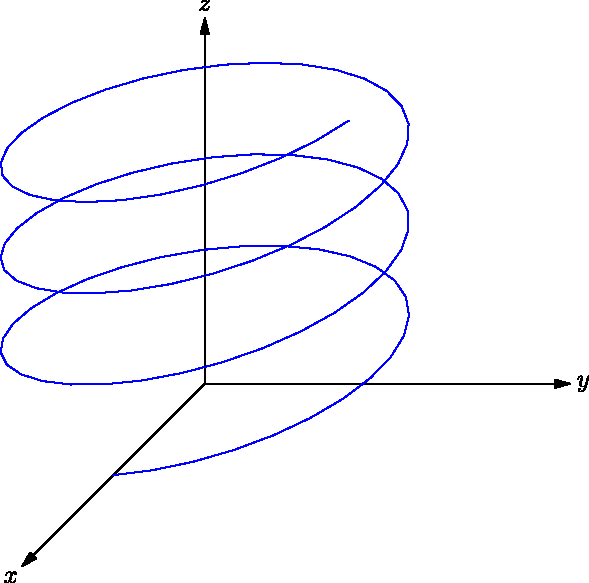
\includegraphics{./cap_curvas/pics/helice}
\caption{\label{helicedex}Hélice circular dextrogira associada à função vetorial do Exemplo~\ref{cap_curvas:exemplo_helice}.}
  \end{center}
\end{figure}

\begin{ex}\label{cap_curvas:exemplo_helice}
A função vetorial $\vct{f}(t)=\cos(t)\vct{i}+\sin(t)\vct{j}+t\vct{k}$ para $ t \in\mathbb{R}$ descreve uma hélice circular, como mostra a figura \ref{helicedex}.
\end{ex}

\begin{exer} Reconheça e represente graficamente as curvas descritas pelas seguintes funções vetoriais:
\begin{itemize}
\item [a)] $\vct{f}(t)=\sin(t)\vct{i}+\cos(t)\vct{j}+\vct{k}$, $0\leq t \leq \pi$
\item [b)] $\vct{f}(t)=\sin(t)\vct{i}+2\cos(t)\vct{k}$, $0\leq t \leq 2\pi$
\item [c)] $\vct{f}(t)=\sin(t)\vct{i}+\cos(t)\vct{k}$, $-\infty < t < \infty$
\item [d)] $\vct{f}(t)=t\vct{i}+\sqrt{4-t^2}~\!\vct{j}$, $-2 \leq t \leq 2$
\item [e)] $\vct{f}(t)=t\vct{i}+\cosh(t)\vct{j}$, $-\infty < t < \infty $
\item [f)] $\vct{f}(t)=\sinh(t)\vct{i}+\cosh(t)\vct{j}$, $-\infty < t< \infty $
\end{itemize} 
Resp: Semicircunferência de raio 1 centrada em $(0,0,1)$ sobre o plano $z=1$. Elipse de semi-eixos $1$ e $2$ centrada na origem sobre o plano $xz$. Hélice circular levogira de raio $1$ e passo $2\pi$.  Semicircunferência de raio 2 centrada na origem sobre o plano $xy$ e $y\geq 0$. Uma catenária sobre o plano $xy$. Uma hipérbole. 
\end{exer}

O limite\index{limite de uma função vetorial de uma variável}, a derivação\index{derivada de uma função vetorial de uma variável} e a integração vetorial\index{integral de uma função vetorial de uma variável} são definidas componente a componente no sistema de coordenadas cartesiano:
\begin{eqnarray}
\lim_{t\to a}\vct{r}(t)&=&\lim_{t\to a}x(t) \vct{i}+\lim_{t\to a}y(t)\vct{j}+\lim_{t\to a}z(t)\vct{k}\label{deflim}\\
\frac{d\vct{r}(t)}{dt}&=&\frac{d x(t)}{dt}\vct{i}+\frac{d y(t)}{dt}\vct{j}+\frac{d z(t)}{dt}\vct{k}\label{defder}\\
\int_{a}^b\vct{r}(t){dt}&=&\int_{a}^bx(t)dt~\!\vct{i}+\int_{a}^by(t)dt~\!\vct{j}+\int_{a}^bz(t)dt~\!\vct{k}\label{defint}\\
\int\vct{r}(t){dt}&=&\int x(t)dt~\!\vct{i}+\int y(t)dt~\!\vct{j}+\int z(t)dt~\!\vct{k}\label{defint2}
\end{eqnarray}

\begin{teo}[Regras de derivação] A derivada de funções vetoriais satisfaz as seguintes identidades:
\begin{enumerate}
\item Se $\vct{r}(t)$ é um vetor constante, então $\vct{r}'(t)=\vct{0}$. 
\item $\frac{d}{dt}\left[\alpha \vct{r}_1(t)+\beta \vct{r}_2(t)\right]=\alpha\frac{d\vct{r}_1(t)}{dt}+\beta\frac{d\vct{r}_2(t)}{dt}$
\item Se $f(t)$ é uma função real, então $\frac{d}{dt}\left[f(t) \vct{r}(t)\right]=f'(t)\vct{r}(t)+f(t)\frac{d\vct{r}(t)}{dt}$
\item $\frac{d}{dt}\left[\vct{r}_1(t)\cdot \vct{r}_2(t)\right]=\vct{r}_1(t)\cdot\frac{d\vct{r}_2(t)}{dt}+\frac{d\vct{r}_1(t)}{dt}\cdot\vct{r}_2(t)$
\item $\frac{d}{dt}\left[\vct{r}_1(t)\times \vct{r}_2(t)\right]=\vct{r}_1(t)\times\frac{d\vct{r}_2(t)}{dt}+\frac{d\vct{r}_1(t)}{dt}\times\vct{r}_2(t)$
\end{enumerate}
\end{teo}
\begin{proof} Os dois primeiros ítens podem ser obtidos diretamente de (\ref{defder}). A verificação fica a cargo do leitor. O item três pode ser obtido de  uma aplicação da regra da cadeia a (\ref{defder})\index{derivada do produto de um escalar por um vetor}:
\begin{eqnarray*}\frac{d}{dt}\left[f(t) \vct{r}(t)\right]&=& \frac{d}{dt}\left[f(t) {x}(t)\vct{i}+f(t) {y}(t)\vct{j}+f(t) {z}(t)\vct{k}\right]\\
&=&\left[f'(t) x(t)+f(t)x'(t)\right]\vct{i}+\left[f'(t) y(t)+f(t)y'(t)\right]\vct{j}+\left[f'(t) z(t)+f(t)z'(t)\right]\vct{k}\\
&=&f'(t)\left[x(t)\vct{i}+y(t)\vct{j}+z(t)\vct{k}\right]+f(t)\left[x'(t)\vct{i}+y'(t)\vct{j}+z'(t)\vct{k}\right]\\
&=&f'(t)\vct{r}(t)+f(t)\vct{r}\!~'(t)
\end{eqnarray*}

A derivada do produto escalar de duas funções vetoriais é dado por:\index{derivada do produto escalar}
\begin{eqnarray*}\frac{d}{dt}\left[\vct{r}_1(t)\cdot \vct{r}_2(t)\right]&=&\frac{d}{dt}\left[x_1(t)x_2(t)+z_1(t)z_2(t)+z_1(t)z_2(t)\right]\\
&=&
\left[x_1'(t)x_2(t)+x_1(t)x_2'(t)\right]+\left[y_1'(t)y_2(t)+y_1(t)y_2'(t)\right]
\\&+&\left[z_1'(t)z_2(t)+z_1(t)z_2'(t)\right]\\&=&\vct{r}_1(t)\cdot\frac{d\vct{r}_2(t)}{dt}+\frac{d\vct{r}_1(t)}{dt}\cdot\vct{r}_2(t)
\end{eqnarray*}
Finalmente a derivada do produto vetorial pode ser obtida de\index{derivada do produto vetorial}:
{\allowdisplaybreaks
\begin{eqnarray*}
\frac{d}{dt}\left[\vct{r}_1(t)\times \vct{r}_2(t)\right]&=&\frac{d}{dt}\left[y_1(t) z_2(t)-z_1(t)y_2(t)\right]\vct{i}\\
&+&\frac{d}{dt}\left[z_1(t) x_2(t)-x_1(t)z_2(t)\right]\vct{j}\\
&+&\frac{d}{dt}\left[x_1(t) y_2(t)-y_1(t)x_2(t)\right]\vct{k}\\
&=&\left[y_1'(t) z_2(t)+y_1(t) z_2'(t)-z_1'(t)y_2(t)-z_1(t)y_2'(t)\right]\vct{i}\\
&+&\left[z_1'(t) x_2(t)+z_1(t) x_2'(t)-x_1'(t)z_2(t)-x_1(t)z_2'(t)\right]\vct{j}\\
&+&\left[x_1'(t) y_2(t)+x_1(t) y_2'(t)-y_1'(t)x_2(t)-y_1(t)x_2'(t)\right]\vct{k}\\
&=&\left[y_1'(t) z_2(t)-z_1'(t)y_2(t)\right]\vct{i}\\
&+&\left[z_1'(t) x_2(t)-x_1'(t)z_2(t)\right]\vct{j}\\
&+&\left[x_1'(t) y_2(t)-y_1'(t)x_2(t)\right]\vct{k}\\
&+&\left[y_1(t) z_2'(t)-z_1(t)y_2'(t)\right]\vct{i}\\
&+&\left[z_1(t) x_2'(t)-x_1(t)z_2'(t)\right]\vct{j}\\
&+&\left[x_1(t) y_2'(t)-y_1(t)x_2'(t)\right]\vct{k}\\
&=&\vct{r}_1(t)\times\frac{d\vct{r}_2(t)}{dt}+\frac{d\vct{r}_1(t)}{dt}\times\vct{r}_2(t)
\end{eqnarray*}
}
\end{proof}
\begin{exer} Dada a função vetorial $\vct{r}(t)=t^2\vct{i}+e^t\vct{j}-2\cos\pi t ~\! \vct{k}$, calcule:
\begin{itemize}
\item [a)] $\displaystyle \lim_{t\to 0} \vct{r}(t)$
\item [b)] $\displaystyle \frac{d \vct{r}(t)}{dt}$
\item [c)] $\displaystyle \vct{r}~\!'(1)$
\item [d)] $\displaystyle \int_0^1 \vct{r}(t)dt$
\item [e)] $\displaystyle \int \vct{r}(t)dt$
\end{itemize}
Resp: $\vct{j}-2\vct{k}$, $\vct{r}'\!~(t)=2t\vct{i}+e^t\vct{j}+2\pi\sin\pi t ~\! \vct{k}$, $\vct{r}'\!~(1)=2\vct{i}+e\vct{j}$, $\frac{1}{3}\vct{i}+(e-1)\vct{j}$, $\left(\frac{1}{3}t^3+C_1\right)\vct{i}+\left(e^t+C_2\right)\vct{j}+\left(-\frac{2}{\pi}\sin\pi t+C_3\right)\vct{k}$

\end{exer}

\begin{exer} Verifique que a função vetorial dada por $\vct{f}(t)=\frac{1-t^2}{1+t^2}\vct{i}+\frac{2t}{1+t^2}\vct{j}$, $-\infty<t<\infty$
representa uma curva contida em uma circunferência no plano $xy$  centrada na origem. Identifique o raio desta circunferência, identifique a curva e isole os quatro quadrantes.

Resp: raio=$1$, centro na origem. $Q1: 0<t<1$, $Q2:t>1$, $Q3:t<-1$, $Q4:-1<t<0$. A curva é a circunferência menos o ponto $\left<-1,0\right>$.

\end{exer}

\begin{exer}Encontre a derivada de cada uma das funções vetoriais do exemplo \ref{exfv1}

Resp: $\vct{f'}(t)=\cos(t)\vct{i}-\sin(t)\vct{j}$,~~ $\vct{g'}(t)= \vct{i}+\sinh(t)\vct{k}$, ~~$\vct{h'}(t)=\cos(t)\vct{i}-\sin(t)\vct{j}+\vct{k}$

\end{exer}

\begin{exer} Mostre as seguintes identidades:
\begin{itemize}
\item[a)] $\displaystyle \frac{d\vct{r}(t)}{dt}\cdot \hat{r}(t)=r'(t)$
\item[b)] $\displaystyle \frac{d}{dt}\left[\vct{r}(t)\times\vct{r}~\!'(t)\right]=\vct{r}(t)\times\vct{r}~\!''(t)$
\item[c)] $\displaystyle \frac{d r(t)}{dt}=\frac{1}{r(t)} \vct{r}(t)\cdot\vct{r}~\!'(t)$
\item[d)] $\displaystyle \frac{d\hat{r}(t)}{dt}=\frac{\vct{r}~\!'(t)}{r(t)}-\frac{\vct{r}(t)\cdot\vct{r}~\!'(t)}{r(t)^3}\vct{r}(t)$
\end{itemize}
Observação: Lembre-se que $\hat{r}(t)=\frac{\vct{r}(t)}{r(t)}$ e $r(t)=\|\vct{r}(t)\|$.

\end{exer}

Demonstraremos agora um importante teorema do cálculo vetorial:
\begin{teo}\label{teodernormacst} Uma função vetorial $\vct{u}(t)$ possui norma constante se e somente se $\vct{u}(t)\cdot\vct{u}\!~'(t)=0$. 
\end{teo}
\begin{proof} Como $\|u\|^2=\vct{u}(t)\cdot\vct{u}(t)$, temos
$$\frac{d \|u\|^2}{dt}=\frac{d}{dt}\left[\vct{u}(t)\cdot\vct{u}(t)\right]=\vct{u}\cdot\frac{d\vct{u}}{dt}+\frac{d\vct{u}}{dt}\cdot\vct{u}=2\vct{u}\cdot\frac{d\vct{u}}{dt}$$
Assim, se $\|u\|$ for constante, a derivada à esquerda é nula e temos $\vct{u}(t)\cdot\vct{u}\!~'(t)=0$. Reciprocamente se $\vct{u}(t)\cdot\vct{u}\!~'(t)=0$, então $\|u\|$ deve ser constante.
\end{proof}
\begin{obs} Uma importante interpretação deste teorema é que se $\vct{v}(t)$ representa a velocidade de uma partícula no instante de tempo $t$, então se o módulo da velocidade $v(t)$ for constante e não nulo então a aceleração $\vct{a}=\vct{v}\!~'(t)$ é perpendicular à velocidade sempre que for não nula.  
\end{obs}




\begin{ex}Seja $\vct{r}(t)$ o vetor posição de uma partícula dado por
$$\vct{r}(t)=a\cos(wt)\vct{i}+a\sin(wt)\vct{j}$$
Calcule o vetor velocidade $\vct{v}$ e o vetor aceleração $\vct{v}$ dados por $\vct{v}=\vct{r}~\!'(t)$ e $\vct{a}=\vct{v}~\!'(t)$.
\end{ex}



 
 \section{Comprimento de arco}
% Dada uma curva parametrizada pela função vetorial $\vct{r}(t)=x(t)\vct{i}+y(t)\vct{j}+z(t)\vct{k}$, $t\in[a,b]$, estamos interessados no problema de calcular o comprimento $L$ do arco de descrito por uma curva $\vct{r}(t)$, $a\leq t\leq b$.
 \begin{figure}\caption{Aproximação poligonal do comprimento do arco}\label{fig_compr_arc}
 \end{figure}

 
 \begin{figure}%{0.35\textwidth}
\begin{center}
    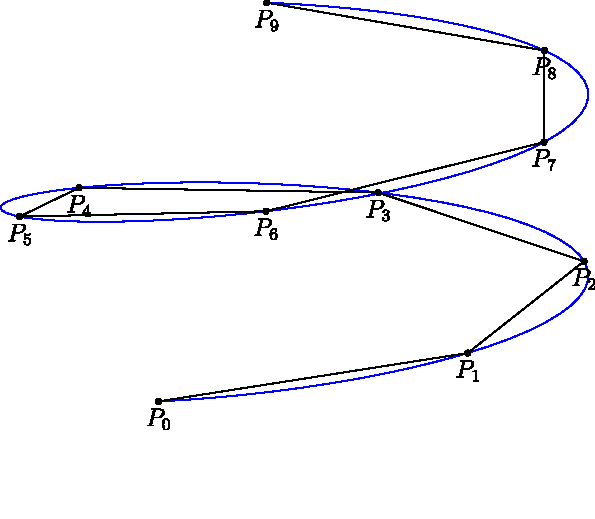
\includegraphics{./cap_curvas/pics/helice_retificacao}
\caption{Aproximação poligonal do comprimento do arco}\label{fig_compr_arc}
  \end{center}
\end{figure}

 
 
Seja $a=t_0<t_1<t_2<\cdots<t_n=b $ uma partição equidistante do domínio com $\Delta t=t_i-t_{i-1}$ e $P_i=\vct{r}(t_i)$, $i=0,1,\cdots,n$, pontos sobre a curva, como mostra a figura \ref{fig_compr_arc}. Uma possível aproximação para o comprimento da curva é dado pelo comprimento da poligonal. Observe que o comprimento do segmento $P_{i-1}P_i$ é dado por $\|P_i-P_{i-1}\|$, logo, a aproximação para o comprimento da curva é
\begin{eqnarray*}
L_n&=&\sum_{i=1}^n\|P_i-P_{i-1}\|\\
&=&\sum_{i=1}^n \sqrt{(x_i-x_{i-1})^2+(y_i-y_{i-1})^2+(z_i-z_{i-1})^2}\\
&=&\sum_{i=1}^n \Delta t \sqrt{\frac{(x_i-x_{i-1})^2}{(\Delta t) ^2}+\frac{(y_i-y_{i-1})^2}{(\Delta t) ^2}+\frac{(z_i-z_{i-1})^2}{(\Delta t) ^2}}\\
&=&\sum_{i=1}^n \sqrt{\left(\frac{x_i-x_{i-1}}{\Delta t }\right)^2+\left(\frac{y_i-y_{i-1}}{\Delta t}\right)^2+\left(\frac{z_i-z_{i-1}}{\Delta t}\right)^2}\Delta t.
\end{eqnarray*}
Naturalmente, $L=\lim_{n\to\infty }L_n$. Como o lado direito da última igualdade é uma soma de Riemann, temos:
\begin{equation}\label{defcomparco}
L=\bigintss_{a}^{b} \sqrt{\left(\frac{dx(t)}{dt}\right)^2+\left(\frac{dy(t)}{dt}\right)^2+\left(\frac{dz(t)}{dt}\right)^2}dt=\int_{a}^{b}\|\vct{r}\!~'(t)\|dt.
\end{equation}
Logo, o comprimero do arco $s$ quando a parâmetro corre de $a$ até $t$ é
\begin{equation}\label{defcomparco_1}
s(t)=\int_{a}^{t}\|\vct{r}\!~'(\tau)\|d\tau,\qquad a\leq t\leq b.
\end{equation}

\section{Triedro de Frenet-Serret}

Seja a curva descrita pela função vetorial $\vct{r}(t)$. Queremos encontrar um vetor que seja tangente à curva em um dado ponto\index{vetor tangente}. Para tal tomamos o limite
$$\lim_{h\to 0} \frac{\vct{r}(t+h)-\vct{r}(t)}{h}$$  
Este limite converge para $\vct{r}'(t)$ e, geometricamente, para o vetor tangente à curva no ponto $P$ relativo a $\vct{r}(t)$\footnote{O leitor atento ao formalismo pode tomar esta coma uma definição de vetor tangente. Adiante, veremos que esta definição é consistente com o vetor tangente do cálculo de funções de uma variável.} sempre que $\vct{r}'(t)\neq \vct{0}$. O sentido do vetor $\vct{r}~\!'(t)$ é dado pela parametrização da curva, em outras palavras, o vetor $\vct{r}~\!'(t)$ aponta no sentido em que o parâmetro $t$ cresce.
% 
% \begin{wrapfigure}{r}{.4\textwidth}
% %\vspace{-40pt}
%  \begin{pspicture}(-.2\textwidth,-.2\textwidth)(.2\textwidth,.2\textwidth)
%  \psset{unit=.15\textwidth}
% % \psset{xunit=.1\textwidth}
%  \newrgbcolor{verde}{0 0.5 0}
%   \psaxes{->,labels=none}(0,0)(-1.2,-1.2)(1.2,1.2)        % sets up axis
%   
%  \pscircle[linecolor=blue,linewidth=1pt](0,0){1}
% 
% \psline[linecolor=verde,linewidth=1pt,arrowscale=2,arrows=->](0.70,0.707)(.30,1.107)
% %\psline[linecolor=verde,linewidth=1pt](.29,1.107)(.40,1.107)
% %\psline[linecolor=verde,linewidth=1pt](.30,1.117)(.30,1.007)
% \psline[linecolor=red,linewidth=1pt,arrowscale=2,arrows=->](0,0)(0.707,0.707)
% %\psline[linecolor=red,linewidth=1pt](0.707,0.707)(0.607,0.707)
% %\psline[linecolor=red,linewidth=1pt](0.707,0.707)(0.707,0.607)
% 
%  \rput[0](0.7,0.5){$\vct{r}(t)$}
% \rput[0](0.55,1.1){$\vct{r}~\!'(t)$}
% 
% \rput[0](1.2,-.1){$x$}
% \rput[0](.07,1.2){$y$} 
% \rput[0](1.05,.1){$1$}
% 
% 
%   % \psplot[linecolor=blue, linewidth=1pt]{0}{2}{x}
%   % \psline[ linecolor=blue, linewidth=1pt](7,0)(7,1)
%  
%  \end{pspicture}\caption{O vetor tangente $\vct{r}\!~'(t)$}\label{circtang}
% \end{wrapfigure}
% 
% 
% \begin{ex}
% Consideramos a circunferência parametrizada conforme a seguinte função vetorial:
% $$\vct{r}(t)=\cos(wt)\vct{i}+\sin(wt)\vct{j},~~ w>0.$$
% A derivada de $\vct{r}(t)$ é dada por
% $$\vct{r}\!~'(t)=-w\sin(wt)\vct{i}+w\cos(wt)\vct{j}.$$
% Veja na figura \ref{circtang}, uma representação gráfica da circunferência, do vetor $\vct{r}(t)$ e de sua derivada $\vct{r}\!~'(t)$. Os vetores $\vct{r}(t)$ e $\vct{r}'(t)$ são ortogonais em função do teorema \ref{teodernormacst}.  A norma de $\vct{r}~\!'(t)$ vale
% \begin{eqnarray*}
% \|\vct{r}~\!'(t)\|\!&=&\!\sqrt{\left[-w\sin(wt)\right]^2+\left[w\cos(wt)\right]^2}\\
% \!&=&\!\sqrt{w^2\left[\sin^2(wt)+\cos^2(wt)\right]}=w
% \end{eqnarray*}
% \end{ex}
% 
% Observe que a norma do vetor tangente depende de como a curva é parametrizada e não apenas da curva em si. A fim de trabalhar com um objeto que independe da parametrização, é natural definirmos o vetor tangente unitário\index{vetor tangente unitário}, denotado por $\vct{T}$ (veja figura \ref{Frenet_Serret}):
% \begin{equation}\label{defvecunit}
% \|\vct{T}(t)\|=\frac{\vct{r}\!~'(t)}{\left\|\vct{r}\!~'(t)\right\|},\qquad \vct{r}\!~'(t)\neq \vct{0}.
% \end{equation} 
% A condição de existência para o vetor $\vct{T}$ é a função vetorial que parametriza a curva seja diferenciável que sua derivada seja diferente de zero, ou seja, que a parametrização seja regular.
% 
% \begin{obs} Quando $\vct{r}(t)$ representa a trajetória de uma partícula ao longo do tempo, a derivada $\vct{r}\!~(t)$ é a velocidade $\vct{v}(t)$ da partícula. Neste caso, o vetor tangente unitário é o versor associado a $\vct{v}(t)$:
% $$\vct{v}(t)=v(t) \hat{v}(t)=v(t) \vct{T}(t).$$
% A norma de $\vct{v}(t)$, denotada por $v(t)$, é chamada de velocidade escalar\index{velocidade escalar}. O vetor $\vct{T}(t)$ indica o sentido e a direção da velocidade.
% \end{obs}
% 
% O vetor $\vct{T}$ pode ser definido de forma alternativa como segue: olhamos $s$ como função de $t$ na expressão (\ref{defcomparco_1}) e observamos que $s'(t)=\|\vct{r}\!~'(t)\|>0$. Assim, $s(t)$ é uma função contínua e monótona de $t$. Também, usando a rega da cadeia, temos:
% $$
% \frac{d\vct{r}}{dt}=\frac{d\vct{r}}{ds}\frac{ds}{dt}=\frac{d\vct{r}}{ds}\|\vct{r}\!~'(t)\|.
% $$
% Como $\vct{r}'(t)$ representa o vetor tangente, então
% $$
% \frac{d\vct{r}}{ds}=\frac{1}{\|\vct{r}\!~'(t)\|}\frac{d\vct{r}}{dt}=\vct{T}
% $$
% representa um vetor tangente unitário.
% 
% \begin{exer}
% Considere as funções vetoriais dadas por
% \begin{eqnarray*}
% \vct{f}(t)&=&\cos(\pi t)\vct{i}+\sin(\pi t)\vct{j}\\
% \vct{g}(t)&=&\cos(\pi t^3)\vct{i}+\sin(\pi t^3)\vct{j}
% \end{eqnarray*}
% Verifique que ambas parametrizam a mesma curva quando $-1\leq t \leq 1$. Verifique se as parametrizações são regulares e compare o comportamento da derivada em $t=0$. Que consequências isso tem para a existência do vetor tangente unitário? 
% \end{exer}
% 
% \begin{wrapfigure}{r}{7cm}
% 
% 
% \begin{pspicture}(-3.5,-1.5)(2.5,4.0)
% 
% \psset{arrowscale=2,arrows=->,viewpoint=20 20 20,Decran=15,lightsrc=20 10 5}
% \defFunction[algebraic]%
% {helice}(t)
% {2*cos(2*t)}{5*sin(2*t)}{t}
% \psSolid[arrows=->,object=courbe,r=0,
% range=3 8,
% linecolor=blue,
% linewidth=0.05,
% resolution=360,
% function=helice]%
% 
%   \pstThreeDLine[linecolor=red,linewidth=1pt,arrows=->](1.9203406,-1.3970775,3.)(2.2653647,1.5669842,3.3087017)
%   \pstThreeDLine[linecolor=red,linewidth=1pt,arrows=->](1.9203406,-1.3970775,3.)(-1.0524784,-1.0330466,2.8272902)
%    \pstThreeDLine[linecolor=red,linewidth=1pt,arrows=->](1.9203406,-1.3970775,3.)(1.7122408,-1.6831192,5.9790728)
%       
%       
%  
%   \pstThreeDLine[linecolor=red,linewidth=1pt,arrows=->](-0.29,4.95,4)(-2.94,3.64,4.53)
%   \pstThreeDLine[linecolor=red,linewidth=1pt,arrows=->](-0.29,4.95,4)(0.6965073,2.1212711,3.7968617)
%   \pstThreeDLine[linecolor=red,linewidth=1pt,arrows=->](-0.29,4.95,4)(0.4292406,4.9891601,6.9119509)
%   
%   
%       
%   \pstThreeDLine[linecolor=red,linewidth=1pt,arrows=->](-1.6781431,-2.7201056,5. )(-0.9299871,-5.6049034,5.3438083)
%     \pstThreeDLine[linecolor=red,linewidth=1pt,arrows=->](-1.6781431,-2.7201056,5. )(1.1989964,-1.9351497,5.3254427)
%     \pstThreeDLine[linecolor=red,linewidth=1pt,arrows=->](-1.6781431,-2.7201056,5. )(-2.0810467,-2.471538,7.9624117)
%   
%   \pstThreeDLine[linecolor=red,linewidth=1pt,arrows=->](0.2734744,4.9530368,7.)(-2.4850089,5.9049461,7.6961596)
%     \pstThreeDLine[linecolor=red,linewidth=1pt,arrows=->](0.2734744,4.9530368,7.)(-0.6596792,2.1083429,7.1921997)
%   \pstThreeDLine[linecolor=red,linewidth=1pt,arrows=->](0.2734744,4.9530368,7.)(0.9945803,4.913222,9.9117728)
%   
%   \psPoint(-2.9,6.1,8){Nome1}
%       \rput*(Nome1){$\vct{T}$}
%   
%   \psPoint(-1,1.5,7.4){Nome2}
%       \rput*(Nome2){$\vct{N}$}
% 
%         \psPoint(1,5,10.4){Nome3}
%       \rput*(Nome3){$\vct{B}$}
% 
%   
%   
%   \axesIIID[linecolor=black](0,0,0)(4.5,4.5,11)
%  \end{pspicture}\caption{Triedro de Frenet-Serret}\label{Frenet_Serret}
%  
% \end{wrapfigure}
% 
% Agora, queremos definir um vetor ortogonal a $\vct{T}$ que esteja no mesmo plano formado por $\vct{r}'(t)$ e $\vct{r}''(t)$. Para isso, usamos o resultado do teorema \ref{teodernormacst}. Observe que a função vetorial $\vct{T}(t)$ possui módulo constante e, portanto, $\vct{T}(t)\cdot \vct{T}'(t)=0$. Observe que $\vct{T}(t)$ e $\vct{T}'(t)$ estão ambos no plano formado por $\vct{r}'(t)$ e $\vct{r}''(t)$ e são ortogonais entre si. No entanto, $\vct{T}'(t)$ não é necessariamente unitário. Logo, faz sentido definir o vetor normal unitário\index{vetor normal unitário} como
% $$
% \vct{N}=\frac{\vct{T}'(t)}{\|\vct{T}'(t)\|}.
% $$
% A figura \ref{Frenet_Serret} apresenta a representação de alguns vetores normais unitários.
% 
% Finalmente, vamos definir um vetor unitário que é simultanemente ortogonal a $\vct{T}$ e $\vct{N}$. A forma natural de obter um vetor ortogonal a outros dois vem do produto vetorial. Assim, o vetor binormal unitário\index{vetor binormal unitário} é definido como
% $$
% \vct{B}=\vct{T}\times\vct{N}.
% $$
% Das propriedades de produto vetorial, temos que $\vct{B}$, além de ortogonal a $\vct{T}$ e $\vct{N}$, é unitário e forma um sistema dextrogiro. O trio $\vct{T}$, $\vct{N}$ e $\vct{B}$ é chamado de triedro de Frenet-Serret. A figura \ref{Frenet_Serret} apresenta a representação de alguns triedros de Frenet-Serret.
% 
% 
% \section{Curvatura e Torção}
% 
% Nessa seção, estamos interessados em definir, a cada ponto da curva, funções que medem o quanto ela está torcida ou curvada, isto é, se a curva é muito diferente de uma reta ou se está fora de qualquer plano do espaço. Primeiro, definiremos uma função chamada de curvatura\index{curvatura}, que mede a cada ponto do domínio, a variação do vetor tangente com respeito ao comprimento de arco $s$. Naturalmente, queremos que a reta tenha curvatura nula, pois ela não difere da sua tangente em ponto algum. Para facilitar a visualização, podemos começar pensando apenas nas curvas que estão contidas em algum plano. A figura \ref{curvatura} nos dá uma ideia de curvatura.
% 
% \begin{figure}[!ht]
% \begin{center}
% \psset{xunit =1cm,yunit=1cm, linewidth=1\pslinewidth}
%  \begin{pspicture}(0,-1)(4,3)
%  
% \psplot[plotstyle=curve,linewidth=2\pslinewidth,linecolor=blue]{0}{3}{x}
% 
% \rput(1.5,-.5){Curvatura nula}
% 
% \end{pspicture}
%  \begin{pspicture}(0,-1)(4,3)
%  
% \psplot[plotstyle=curve,linewidth=2\pslinewidth,linecolor=blue]{0}{3}{x x mul 3 div}
% 
% \rput(1.5,-.5){Curvatura pequena}
% 
% \end{pspicture}
%  \begin{pspicture}(-2,-2)(2,2)
%  
% \parametricplot[plotstyle=curve,linewidth=2\pslinewidth,linecolor=blue]{0}{360}{3 t mul cos 2.718 -0.01 t mul exp mul 3 t mul sin 2.718 -0.01 t mul exp mul 2 mul}
% 
% \rput(0,-1.5){Curvatura grande}
% 
% \end{pspicture}
% 
% 
% \end{center}
% \caption{Ideia de curvatura.\label{curvatura}}
% \end{figure}
% 
% Pelo teorema \ref{teodernormacst}, temos que $\frac{d \vct{T} }{ds}$ é paralelo ao vetor normal $\vct{N}$, ou seja,
% \begin{equation}{\label{Frenet_1}}
% \frac{d \vct{T} }{ds}=\kappa   \vct{N},
% \end{equation}
% onde $\kappa(t)>0$ é uma função escalar chamada de curvatura. Por outro lado, calculamos a variação do vetor tangente com respeito ao comprimento de arco $s$ usando a regra da cadeia
% $$
% \frac{d \vct{T} }{ds}=\frac{d \vct{T} }{dt}\frac{dt}{ds}=\frac{d \vct{T} }{dt}\frac{1}{|s'(t)|},
% $$
% onde $s(t)$ é a função que mede o comprimento do arco dado pela expressão (\ref{defcomparco_1}). Usando o fato que $s'(t)=\|\vct{r}'(t)\|$, temos:
% $$
% \frac{d \vct{T} }{ds}=\frac{1}{\|\vct{r}'(t)\|}\frac{d \vct{T} }{dt}.
% $$
% Portanto, podemos escrever
% $$
% \kappa(t)=\frac{\|\vct{T}'(t)\|}{\|\vct{r}'(t)\|}.
% $$
% 
% Definimos também, para cada ponto $t$ do domínio, o raio de curvatura\index{raio de curvatura} $\rho(t)$ da forma:
% $$
% \rho(t)=\frac{1}{\kappa(t)}.
% $$
% O raio de curvatura tem a seguinte interpretação geométrica: considere um ponto $\vct{r}(t_0)$ onde da curvatura não é nula e defina o ponto $\vct{r}(t_0)+\kappa(t_0)\vct{N}$, chamado de centro de curvatura\index{centro de curvatura}. O círculo centrado no centro de curvatura e raio $\rho(t_0)$ é tangente a curva em $t_0$ e possui a mesma curvatura (veja a figura \ref{raio_de_curvatura}).
% 
% \begin{wrapfigure}{r}{9cm}
% 
% \begin{pspicture}(-6,-2)(3,7)
%   \psaxes{->}(0,0)(-5,-1)(2.5,6.5)        % sets up axis
% \psplot[plotstyle=curve,linewidth=2\pslinewidth,linecolor=blue]{-2}{2}{x x mul}
% 
% \parametricplot[algebraic=true,plotstyle=curve,linewidth=2\pslinewidth,linecolor=red]{-1}{.6}{-3.999848+5.59*cos(t),5.59*sin(t)+3.499924}
% 
% \rput(-4,3.2){Centro de curvatura}
%  \pscircle[algebraic=true,plotstyle=curve,linewidth=2\pslinewidth,linecolor=red](-3.999848,3.499924){.05}
% \end{pspicture}
% 
% \caption{Círculo de curvatura}\label{raio_de_curvatura}
% 
% \end{wrapfigure}
% \begin{exer}Calcule a curvatura da curva $\vct{r}=a\cos(t)\vct{i}+a\sin(t)\vct{j},\qquad a>0,\ 0\leq t\leq 2\pi$.
% \end{exer}
% \begin{ex}Dada a curva $y=x^2$, vamos encontrar a curvatura e o raio de curvatura no ponto $x=1$. Primeiro, encontramos uma parametrização para essa curva, por exemplo, $\vct{r}=t\vct{i}+t^2\vct{j}$. Calculamos:
% $$
% \vct{r}'=\vct{i}+2t\vct{j},
% $$
% $$
% \|\vct{r}'\|=\sqrt{1+4t^2},
% $$
% $$
% \vct{T}=\frac{1}{\sqrt{1+4t^2}}\left(\vct{i}+2t\vct{j}\right)
% $$
% e
% $$
% \vct{T}'=-\frac{4t}{\sqrt{(1+4t^2})^3}\vct{i}+\left(-\frac{8t^2}{\sqrt{(1+4t^2})^3}+\frac{2}{\sqrt{1+4t^2}}\right)\vct{j},
% $$
% Em $t=1$, temos:
% $$
% \|\vct{r}'\|=\sqrt{5},
% $$
% $$
% \vct{T}'=-\frac{4}{\sqrt{5^3}}\vct{i}+\left(-\frac{8}{\sqrt{5^3}}+\frac{2}{\sqrt{5}}\right)\vct{j}=-\frac{4}{\sqrt{5^3}}\vct{i}+\frac{2}{\sqrt{5^3}}\vct{j},
% $$
% e
% $$
% \|\vct{T}'\|=\sqrt{\frac{16}{5^3}+\frac{4}{5^3}}=\frac{2}{5}.
% $$
% Portanto,
% $$
% \kappa(1)=\frac{\|\vct{T}'\|}{\|\vct{r}'\|}=\frac{2}{5\sqrt{5}}
% $$
% e
% $$
% \rho(1)=\frac{5\sqrt{5}}{2}.
% $$
% veja representação geométrica na figura \ref{raio_de_curvatura}.
% \end{ex}
% 
% O leitor deve ter observado que conhecendo somente a curvatura não é possível reconstruir uma curva a partir de um ponto dado. Um curva pode não estar contida em plano algum no espaço e, por isso, precisamos definir uma função escalar, chamada torção, que mede a magnitude da variação do vetor binormal. A figura \ref{torcao} apresenta uma ideia de torção\index{torção}: uma curva contida em algum plano no espaço tem torção nula e quando maior a variação com respeito ao plano definido por $\vct{T}$ e $\vct{N}$, maior a torção. O leitor deve tomar cuidado na interpretação da figura \ref{torcao}, pois se esticarmos indefinidamente a hélice circular representada, ela voltará a se aproximar de uma reta, que tem torção nula (veja problema \ref{prob_torcao}). Sabendo que a torção será definida em termos da variação do vetor binormal com respeito ao comprimento de arco $s(t)$, fazendo algumas observações:
% $$
% \frac{d\vct{B}}{ds}=\frac{d}{ds}\left(\vct{T}\times\vct{N}\right)=\frac{d\vct{T}}{ds}\times \vct{N}+\vct{T}\times\frac{d\vct{N}}{ds}.
% $$
% Usando a expressão (\ref{Frenet_1}), temos que $\frac{d\vct{T}}{ds}=\kappa\vct{N}$, logo 
% $$
% \frac{d\vct{B}}{ds}=\vct{T}\times\frac{d\vct{N}}{ds}.
% $$
% Isso implica que $\frac{d\vct{B}}{ds}$ é ortogonal a $\vct{T}$. Mas, pelo teorema \ref{teodernormacst}, temos que $\frac{d\vct{B}}{ds}$ é ortogonal a $\vct{B}$. Logo, $\frac{d\vct{B}}{ds}$ é paralelo a $\vct{N}$, ou seja,
% \begin{equation}{\label{Frenet_2}}
% \frac{d\vct{B}}{ds}=-\tau\vct{N},
% \end{equation}
% onde $\tau$ é chamado de torção\index{torção}. O sinal negativo tem um propósito: quando $\tau>0$, $\frac{d\vct{B}}{ds}$ está no sentido de $-\vct{N}$; então se $P$ é um ponto sobre a curva movendo-se no sentido positivo, $\vct{B}$ gira em torno de $\vct{T}$ como um parafuso de rosca direita sendo apertado (veja a figura \ref{Curvatura_torcao_1}). Em alguns contextos, calculamos a módulo da torção, dada por
% $$
% |\tau|=\left\|\frac{d\vct{B}}{ds}\right\|=\frac{\|\vct{B}'(t)\|}{\|\vct{r}'(t)\|}.
% $$
% 
% \begin{figure}[!ht]
% \begin{center}
% \psset{xunit =1cm,yunit=1cm, linewidth=1\pslinewidth}
% \begin{pspicture}(-2.5,-2.0)(2.5,4.0)
% \psset{viewpoint=20 20 20,Decran=15,lightsrc=20 10 5}
% \defFunction[algebraic]%
% {helice}(t)
% {2*cos(2*t)}{5*sin(2*t)}{0}
% \psSolid[arrows=->,object=courbe,r=0,
% range=0 5,
% linecolor=blue,
% linewidth=0.05,
% resolution=360,
% function=helice]%
% \rput(1.0,-1.8){Torção nula}
%   \axesIIID[linecolor=black](0,0,0)(4.5,6,5)
% \end{pspicture}
% \begin{pspicture}(-2.5,-2.0)(2.5,4.0)
% \psset{viewpoint=20 20 20,Decran=15,lightsrc=20 10 5}
% \defFunction[algebraic]%
% {helice}(t)
% {2*cos(2*t)}{5*sin(2*t)}{t/4}
% \psSolid[arrows=->,object=courbe,r=0,
% range=0 4,
% linecolor=blue,
% linewidth=0.05,
% resolution=360,
% function=helice]%
% \rput(1.0,-1.8){Torção pequena}
%   \axesIIID[linecolor=black](0,0,0)(4.5,6,5)
% \end{pspicture}
% \begin{pspicture}(-2.5,-2.0)(2.5,4.0)
% \psset{viewpoint=20 20 20,Decran=15,lightsrc=20 10 5}
% \defFunction[algebraic]%
% {helice}(t)
% {2*cos(2*t)}{5*sin(2*t)}{2*t}
% \psSolid[arrows=->,object=courbe,r=0,
% range=0 4,
% linecolor=blue,
% linewidth=0.05,
% resolution=360,
% function=helice]%
% \rput(1.0,-1.8){Torção grande}
%   \axesIIID[linecolor=black](0,0,0)(4.5,6,7)
% \end{pspicture}
% 
% \end{center}
% \caption{Ideia de torção.\label{torcao}}
% \end{figure}
% Ainda, definimos o raio de torção\index{raio de torção} por
% $$
% \sigma(t)=\frac{1}{\tau(t)}.
% $$
% 
% Podemos calcular $\frac{d\vct{N}}{ds}$ em termos da curvatura e da torção:
% \begin{equation*}
% \frac{d\vct{N}}{ds}=\frac{d}{ds}\left(\vct{B}\times\vct{T}\right)=\frac{d\vct{B}}{ds}\times \vct{T}+\vct{B}\times\frac{d\vct{T}}{ds}.
% \end{equation*}
% Usando as expressões (\ref{Frenet_1}) e (\ref{Frenet_2}), escrevemos
% \begin{equation*}
% \frac{d\vct{N}}{ds}=-\tau\vct{N} \times \vct{T}+\vct{B}\times \kappa \vct{N}.
% \end{equation*}
% ou seja,
% \begin{equation}{\label{Frenet_3}}
% \frac{d\vct{N}}{ds}=-\kappa \vct{T}+\tau \vct{B}.
% \end{equation}
% As equações (\ref{Frenet_1}), (\ref{Frenet_2}) e (\ref{Frenet_3}) são chamadas de Fórmulas de Frenet-Serret.
% 
% Como esperávamos, se $\kappa=0$, então $\frac{d\vct{T}}{ds}=\vct{0}$, o que implica que $\vct{T}$ não varia ao longo da curva, ou seja, a curva é uma reta. Agora, se $\tau=0$, então $\frac{d\vct{B}}{ds}=\vct{0}$ e $\vct{B}$ é um vetor constante. Como $\vct{B}\cdot \vct{T}=\vct{B}\cdot \frac{d\vct{r}}{ds}=0$, então podemos integrar para obter $\vct{B}\cdot (\vct{r}-\vct{r_0})=0$, onde $r_0$ é um vetor constante da integração. Logo $\vct{r}$ está contido no plano ortogonal a $\vct{B}$.
% 
% 
% 
% \begin{ex} Vamos calcular curvatura, raio de curvatura e o módulo da torção para a hélice circular $\vct{r}(t)=\cos(t)\vct{i}+\sin(t)+t\vct{k}$:
% $$
% \vct{r}'(t)=-\sin(t)\vct{i}+\cos(t)+\vct{k},
% $$
% $$
% \|\vct{r}'(t)\|=\sqrt{2},
% $$
% $$
% \vct{T}(t)=-\frac{\sin(t)}{\sqrt{2}}\vct{i}+\frac{\cos(t)}{\sqrt{2}}+\frac{1}{\sqrt{2}}\vct{k},
% $$
% $$
% \vct{T}'(t)=-\frac{\cos(t)}{\sqrt{2}}\vct{i}-\frac{\sin(t)}{\sqrt{2}},
% $$
% $$
% \|\vct{T}'(t)\|=\frac{1}{\sqrt{2}},
% $$
% $$
% \kappa(t)=\frac{1}{\sqrt{2}}\cdot \frac{1}{\sqrt{2}}=\frac{1}{2},
% $$
% $$
% \rho(t)=2,
% $$
% $$
% \vct{N}(t)=-\cos(t)\vct{i}-\sin(t)\vct{j},
% $$
% \begin{eqnarray*}
% \vct{B}(t)&=&\left|\begin{array}{ccc}\vct{i}&\vct{j}&\vct{k}\\-\frac{\sin(t)}{\sqrt{2}}&\frac{\cos(t)}{\sqrt{2}}&\frac{1}{\sqrt{2}}\\-\cos(t)&-\sin(t)&0\end{array}\right|\\
% &=&\frac{\sin(t)}{\sqrt{2}}\vct{i}-\frac{\cos(t)}{\sqrt{2}}\vct{j}+\frac{1}{\sqrt{2}}\vct{k}.
% \end{eqnarray*}
% $$
% \vct{B}'(t)=\frac{\cos(t)}{\sqrt{2}}\vct{i}+\frac{\sin(t)}{\sqrt{2}}\vct{j},
% $$
% $$
% \|\vct{B}'(t)\|=\frac{1}{\sqrt{2}},
% $$
% $$
% |\tau(t)|=\frac{1}{2}.
% $$
% \end{ex}
% 
% \begin{exer} Calcule a curvatura, o raio de curvatura e o módulo da torção das curvas abaixo:
% \begin{itemize}
% \item[a)] $\vct{r}=a\cosh(t)\vct{i}+b\sinh(t)\vct{j}$, $-\infty<t<\infty$, $a>0,\ b>0$.
% \item[b)] $\vct{r}=a\cos(t)\vct{i}+b\sin(t)\vct{k}$, $0\leq t\leq 2\pi$, $a>0,\ b>0$.
% \item[c)] $\vct{r}=a\cos(t)\vct{i}+a\sin(t)+ct\vct{k}$, $t\geq 0$, $a>0,\ c>0$.
% 
% \end{itemize}
% \end{exer}
% 
% \begin{exer}{\label{prob_torcao}} Dada a hélice circular $\vct{r}=a\cos(t)\vct{i}+a\sin(t)+ct\vct{k}$, $t\geq 0$, $a>0,\ c>0$, calcule o valor de $c$ para que a torção seja máxima.
% \end{exer}
% 
% \begin{wrapfigure}{r}{8cm}
% \begin{pspicture}(-1.0,2)(6.5,8.0)
% 
% \psset{arrowscale=2,arrows=->,viewpoint=12 12 12,Decran=15,lightsrc=20 10 5}
% \defFunction[algebraic]%
% {helice}(t)
% {2*cos(2*t)}{5*sin(2*t)}{t}
% \psSolid[arrows=->,object=courbe,r=0,
% range=6.5 8,
% linecolor=blue,
% linewidth=0.05,
% resolution=360,
% function=helice]%
%        
%   \pstThreeDLine[linecolor=red,linewidth=1pt,arrows=->](0.2734744,4.9530368,7.)(-2.4850089,5.9049461,7.6961596)
%     \pstThreeDLine[linecolor=red,linewidth=1pt,arrows=->](0.2734744,4.9530368,7.)(-0.6596792,2.1083429,7.1921997)
%     \pstThreeDLine[linecolor=green,linewidth=1pt,arrows=->](0.2734744,4.9530368,7.)(1.206628,7.7977307,6.8078003)
%     
%   \pstThreeDLine[linecolor=red,linewidth=1pt,arrows=->](0.2734744,4.9530368,7.)(0.9945803,4.913222,9.9117728)
%   %\pstThreeDCoor[IIIDticks]
%   \pstThreeDEllipse[beginAngle=0,endAngle=90,linestyle=dashed](0.27,5,7.)(-2.55,1.4,0.6)(0.1,-2.0,0.19)
%     \pstThreeDEllipse[beginAngle=0,endAngle=90,linestyle=dashed](0.4,6.2,8.5)(0.7211059,0.0,2.911772)(0.9,3.5,-1.2)
%     
%  %    \pstThreeDLine[linecolor=green,linewidth=1pt,arrows=->](0,0,0)(3,0,0)
%   %  \pstThreeDEllipse[beginAngle=0,endAngle=90](0,0,0)(3,0,0)(0,3,0)
%   
%   \psPoint(-2.9,6.0,7.2){Nome1}
%       \rput*(Nome1){$\vct{T}$}
%   
%   \psPoint(-1,1.5,7.3){Nome2}
%       \rput*(Nome2){$\vct{N}$}
% 
%         \psPoint(1.5,8.2,6.8){Nome2a}
%       \rput*(Nome2a){$-\vct{N}$}
% 
%       
%         \psPoint(1,5,10.2){Nome3}
%       \rput*(Nome3){$\vct{B}$}
% 
%       
%               \psPoint(-2.4,5.5,8.0){Nome4}
%       \rput*(Nome4){Curvatura}
% 
%               \psPoint(1.5,7.5,7.5){Nome5}
%       \rput*(Nome5){Torção}
% 
%       \psPoint(3.5,4,7.1){Nome6}
%       \rput*(Nome6){$\vct{r}(t)$}
%       
% %  \axesIIID[linecolor=black](0,0,0)(4.5,4.5,11)
%  \end{pspicture}\caption{Curvatura e Torção}\label{Curvatura_torcao_1}
%  
% \end{wrapfigure}
% 
% A curvatura e a torção podem ser calculadas de maneira mais simples. Para concluir isso, começamos calculando as derivadas de $\vct{r}$. Usamos aqui que $s'(t)=\|\vct{r}'(t)\|$, obtida da equação (\ref{defcomparco_1}):
% $$
% \vct{r}'=\frac{d\vct{r}}{ds}\frac{ds}{dt}=s' \vct{T},
% $$
% \begin{eqnarray*}
% \vct{r}''&=&s'' \vct{T}+s' \vct{T}'\\&=&s'' \vct{T}+s' \|\vct{T}'\|\vct{N}\\
% &=&s'' \vct{T}+s'^2 \kappa \vct{N}
% \end{eqnarray*}
% e
% \begin{eqnarray*}
% \vct{r}'''&=&s''' \vct{T}+s''\vct{T}'+2s's''\kappa \vct{N}+s'^2 \left(\kappa \vct{N}'+\kappa' \vct{N}\right)\\
% &=&s''' \vct{T}+s''s'\kappa \vct{N}+\left(2s's''\kappa+s'^2\kappa'\right) \vct{N}\\
% &+&s'^3 \kappa (-\kappa \vct{T}+\tau\vct{B})\\
% &=&\left(s'''-\kappa^2s'^3\right) \vct{T}+\left(3s''s'\kappa +s'^2\kappa'\right)\vct{N}+s'^3 \kappa \tau\vct{B},
% \end{eqnarray*}
% onde usamos as expressões (\ref{Frenet_1}) e (\ref{Frenet_3}). Agora, tomamos os seguintes produtos:
% $$
% \vct{r}'\times \vct{r}''=s'^3\kappa \vct{B}\qquad\text{e}\qquad
% \vct{r}'\times \vct{r}''\cdot \vct{r}'''=s'^6\kappa^2\tau.
% $$
% Isso implica em 
% $$
% \|\vct{r}'\times \vct{r}''\|=|s'|^3\kappa\qquad\text{e}\qquad
% \vct{r}'\times \vct{r}''\cdot \vct{r}'''=\|\vct{r}'\times \vct{r}''\|^2\tau.
% $$
% ou seja,
% \begin{equation}{\label{curvatura_2}}
% \kappa =\frac{\|\vct{r}'\times \vct{r}''\|}{\|r'\|^3}
% \end{equation}
% e
% \begin{equation}{\label{torcao_2}}
% \tau=\frac{\vct{r}'\times \vct{r}''\cdot \vct{r}'''}{\|\vct{r}'\times \vct{r}''\|^2}.
% \end{equation}
% 
% \begin{obs}Uma aplicação natural é a decomposição da aceleração em suas componentes tangencial e normal. Observe que
% $$
% \vct{r}'=\vct{v}=v\vct{T}=s' \vct{T}
% $$
% e
% $$
% \vct{a}=v' \vct{T}+v^2 \kappa \vct{N}.
% $$
% Concluímos que a aceleração está no plano normal a $\vct{B}$ e possui componentes tangencial e normal:
% $$
% \vct{a}=a_T \vct{T}+a_N \vct{N},
% $$
% onde $a_T=v'$ e $a_N=v^2\kappa$. Então, se a velocidade possui normal constante, temos que $v'=0$ e a aceleração possui apenas componente normal.
% 
% \end{obs}
% \begin{exer}Calcule curvatura e torção para a curva $\vct{r}=a\cos(t)\vct{i}+a\sin(t)\vct{j}+ct\vct{k}$, $a>0$, $c>0$, $t>0$ usando as expressões (\ref{curvatura_2}) e (\ref{torcao_2}).
% \end{exer}
% 
% \begin{ex}Uma motocicleta percorre uma trajetória circular de raio $20m$ com velocidade constante em módulo. A motocicleta poderá derrapar se a aceleração normal exceder $2m/s^2$. Qual é a velocidade máxima do motocicleta para que ela não derrape?
% \end{ex}
% 
% \begin{ex} Consideremos agora, a curva gerada pelas seguintes equações paramétricas:
% $$x(t)=\cos(t)\qquad y(t)=\sin(t)\qquad z(t)=f(t).$$
%  Onde $f(t)$ é uma função dada. Observe que a projeção desta curva no plano $xy$ é uma circuferência de raio 1. A curva é, portanto, gerada pela trajetória de ponto cuja projeção do movimento no plano $xy$ é cirvular e a altura é dada pela função $f(t)$. Podemos calcular a curvatura e a torção conforme a seguir:
%  \begin{eqnarray*}
%   \vec{r}(t)&=&\cos(t)\vec{i}+\sin(t)\vec{j}+f(t)\vec{k}\\
%   \vec{r'}(t)&=&-\sin(t)\vec{i}+\cos(t)\vec{j}+f'(t)\vec{k}\\
%   \vec{r''}(t)&=&-\cos(t)\vec{i}-\sin(t)\vec{j}+f''(t)\vec{k}\\
%   \vec{r'''}(t)&=&\sin(t)\vec{i}-\cos(t)\vec{j}+f'''(t)\vec{k}
%  \end{eqnarray*}
% Assim, calculamos:
%  \begin{eqnarray*}
%   \vec{r'}(t)\times\vec{r''}(t) &=&\left[f''(t)\cos(t)+f'(t)\sin(t)\right]\vec{i}+\left[-f'(t)\cos(t)+f''(t)\sin(t)\right]\vec{j}+\vec{k}\\
%  \vec{r'}(t)\times\vec{r''}(t)\cdot r'''(t)&=&f'(t)+f'''(t)\\
%  \|\vec{r'}(t)\times\vec{r''}(t)\|&=&\sqrt{1+\left(f'(t)\right)^2+\left(f''(t)\right)^2}\\
%  \|\vec{r'}(t)\|&=&\sqrt{1+\left(f'(t)\right)^2}
%  \end{eqnarray*}
% E finalmente, obtemos:
%  \begin{eqnarray*}
% \kappa&=&\frac{\sqrt{1+\left(f'(t)\right)^2+\left(f''(t)\right)^2}}{\left({1+\left(f'(t)\right)^2}\right)^{3/2}}\\
% \tau&=&\frac{f'(t)+f'''(t)}{1+\left(f'(t)\right)^2+\left(f''(t)\right)^2}
%  \end{eqnarray*}
% Podemos, agora, explorar diversos casos particular:
% \begin{itemize}
%  \item [a)] Caso $f(t)=c$ constante. Neste caso, recaímos na circunferência de raio 1, cuja curvatura é 1 e a torção é nula.
%  \item [b)] Caso $f(t)=ct$ com $c$ constante. Recaímos na hélice cicular uniforme, já estudada, cuja curvatura é $\frac{1}{1+c^2}$ e a torção é $\frac{c}{1+c^2}$.
%  \item [c)] Caso $f(t)=ct^2$ com $c$ constante. Recaímos na hélice cicular com espaçamento linearmente crescente, cuja curvatura é dada por ${\frac {\sqrt {4\,{c}^{2}+1+4\,{c}^{2}{t}^{2}}}{ \left( 1+4\,{c}^{2}{t
% }^{2} \right) ^{3/2}}}$ e cuja torção é dada por $2\,{\frac {ct}{4\,{c}^{2}+1+4\,{c}^{2}{t}^{2}}}$.
%  \item [d)] Caso $f(t)=\sin(t)$. Recaímos na elipse de semieixos $1$ e $\sqrt{2}$ no plano $y=z$. Neste caso, a curvatura é $\kappa=\frac{\sqrt{2}}{\left(1+\cos(t)^2\right)^{3/2}}$ e a torção é nula.
%  \item [e)] Caso $\tau=0$, isto é, $f'(t)+f'''(t)=0$, o que é equivalente a $f(t)=a+b\cos(t)+c\sin(t)$ onde $a$, $b$ e $c$ são constantes. Recaímos na elipse de semieixos $1$ e $\sqrt{1+b^2+c^2}$ no plano $z=bx+cy$. Neste caso, a curvatura é $\kappa={\frac {\sqrt {b^2+c^2+1}}{\left(1-bc\sin(2t)+c^2\cos^2(t)+b^2\sin^2(t) \right) ^{3/2}}}$ e a torção é nula.
%   \end{itemize}
% 
%  
%  
% \end{ex}
% 
% 
% 
% 
% 
%\end{document}
%Este trabalho está licenciado sob a Licença Creative Commons Atribuição-CompartilhaIgual 3.0 Não Adaptada. Para ver uma cópia desta licença, visite https://creativecommons.org/licenses/by-sa/3.0/ ou envie uma carta para Creative Commons, PO Box 1866, Mountain View, CA 94042, USA.
% !TEX root = ../main.tex
\chapter{Superfícies}
Neste capítulo, estudaremos funções vetoriais do tipo $\vec{f}(u,v)$, ou seja, uma função que associa um ponto do plano real a vetores no espaço.
\section{Funções vetoriais de duas variáveis reais - superfícies}
Uma função vetorial de duas variáveis é uma função da forma $$\vec{r}:D_1\times D_2 \to \mathbb{R}^3,$$ onde $D_1\times D_2\subseteq \mathbb{R}^2$ é o domínio de definição de $\vec{r}$ e $(u,v)\in D_1\times D_2$ são os parâmetros ou as coordenadas de superfície. Em coordenadas cartesianas, uma função vetorial assume a seguinte forma:
$$\vec{r}(u,v)=x(u,v)\vec{i}+y(u,v)\vec{j}+z(u,v)\vec{k}$$
\begin{ex}\label{exfv_1} São exemplos de funções vetoriais
\begin{itemize}
\item [a)] $\vec{f}(u,v)=\sin(u)\vec{i}+\cos(v)\vec{j}+uv\vec{k}$
\item [b)] $\vec{g}(u,v)=\sin(u)\cos(v) \vec{i}+\cosh(u)\sinh(v)\vec{j}+u\vec{k}$
\end{itemize}
\end{ex}
Uma superfície\index{superfície} no espaço pode ser representada pelo conjunto de pontos de uma função vetorial $\vec{r}(u,v)$ não constante em todo o seu domínio. A seguinte interpretação ajuda entender essa função: se fixamos $v$ e temos que $\vec{r}(u,v)$ descreve uma curva e $\vec{r}_u(u,v)$ é um vetor tangente a essa curva. Da mesma forma, se fixamos $u$ temos que $\vec{r}(u,v)$ descreve uma curva e $\vec{r}_v(u,v)$ é um vetor tangente a essa curva. Se essas curvas não forem paralelas, temos um sistema de coordenadas curvilíneo para escrever todos os pontos da superfície. Pense no globo terrestre, o medidiano de Greenwich e a linha do Equador: o globo como uma superfície, Greenwich e Equador como duas curvas e longitude e latitude como um sistema de coordenadas curvilíneo, veja Figura~\ref{cap_superficies_esfera} Observe que esse sistema curvilíneo fica bem definido quando $\vec{r}_u$ e $\vec{r}_v$ não são paralelos nos pontos do domínio. Chamamos de superfície regular aquela que satisfaz
$$
\vec{r}_u\times \vec{r}_v\neq \vec{0}.
$$
\begin{ex}A função vetorial
$$
\vec{r}=a\sin(u)\cos(v)\vec{i}+a\sin(u)\sin(v)\vec{j}+a\cos(u)\vec{k},~~ a>0, ~ 0\leq u< \pi, ~ 0\leq v< 2\pi
$$
descreve uma esfera centrada na origem e raio $a$. De fato, colocando $$x=a\sin(u)\cos(v),\qquad y=a\sin(u)\sin(v)\qquad\text{e}\qquad z=a\cos(u),$$
temos que
$$
x^2+y^2+z^2=a^2.
$$
Além disso, se $(x,y,z)$ é um ponto qualquer nesta esfera, então existem $u$ e $v$ na parametrização. Para tal, basta escolher $u=\cos^{-1}\left(\frac{z}{a}\right)$ e escolher $v\in[0,2\pi)$ tal que:
$$\cos(v)=\frac{x}{a\sin(u)} \quad \hbox{e} \quad \sin(v)=\frac{y}{a\sin(u)},~~u\neq 0 ~~ \hbox{e} ~~u\neq \pi.$$

 \begin{figure}%{r}{8cm}
\centering
 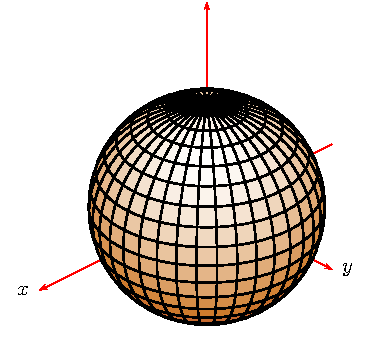
\includegraphics{cap_superficies/figs/figura_1}\label{cap_superficies_esfera}
\caption{Um esfera centrada na origem com meridianos e paralelos traçados.}
\end{figure}
\end{ex}

\begin{ex}A função vetorial
 $$
 \vec{r}=\cosh(u)\cos( v)\vec{i}+ \cosh(u)\sin(v)\vec{j}+\sinh(u)\vec{k},\ 0\leq v\leq 2\pi,\ u\in\mathcal{R}
 $$
 descreve um hiperbolóide de uma folha. De fato, para cada par $(u,v)$ no domínio, a parametrização
 $$
 x(u,v)=\cosh(u)\cos(v),\qquad y(u,v)=\cosh(u)\sin(v)\quad\text{e}\quad z(u,v)=\sinh(u)
 $$
 nos leva na equação canônica de um hiperbolóide de uma folha:
 \begin{eqnarray*}
 x^2+y^2-z^2&=&\cosh^2(u)\cos^2(v)+\cosh^2(u)\sin^2(v)-\sinh^2(u)  \\
 &=&\cosh^2(u)(\cos^2(v)+\sin^2(v))-\sinh^2(u)  \\
 &=&\cosh^2(u)-\sinh^2(u)  \\
 &=&1.
 \end{eqnarray*}
Recriprocamente, se $(x,y,z)$ é um ponto sobre o hiperbolóide, definimos $u=\sin^{-1}(z)$ e escolhemos $v\in[0,2\pi)$ tal que:
$$\cos(v)=\frac{x}{\cosh(u)} \quad \hbox{e} \quad \sin(v)=\frac{y}{\cosh(u)}.$$
 \end{ex}
 
 \subsection*{Exercícios}
 \begin{exer}Mostre que a função vetorial
  $$
  \vec{r}(u,v)=(u+v)\vec{i}+(u-v)\vec{j}+(3u-2v+1)\vec{k}, \qquad 0\leq u,v\leq \infty,
  $$
  descreve um plano.
 \end{exer}

 \begin{exer}Mostre que a função vetorial
  $$
  \vec{r}(u,v)=3\cos(u)\vec{i}+3\sin(u)\vec{j} +v\vec{k}, \qquad 0\leq u\leq 2\pi,\quad 0\leq v\leq 2
  $$
  descreve um cilíndro.
 \end{exer}
 
 
\section{Vetor unitário normal e orientação}\index{vetor normal à uma superfície}
Para os fins de teoria de integraçao sobre superfícies, que discutiremos mais adiante, é fundamental definir o vetor unitário normal. Dado uma superfície e um ponto nela, dizemos que um vetor é normal à superfície se ele é perpendicular no ponto a cada curva contida na superfícies. Em especial, um vetor normal à superfícies no ponto $x_0=x(u_0,v_0)$, $y_0=y(u_0,v_0)$ e $z_0=z(u_0,v_0)$, deve ser perpendicular às curvas $\vec{r}(u_0,v)$ e $\vec{r}(u,v_0)$, isto é, as curvas geradas quando se fixa um dos parâmetros $u_0$ ou $v_0$, respectivamente. Assim, podemos concluir que cada vetor normal está da mesma direção do produto vetorial $\vec{r}_u\times\vec{r}_v$. Finalmente, o vetor normal unitário deve ter norma unitária, portanto, deve ser da forma:
\begin{equation}\label{cap_superficies_normal_unitario}
 \vec{n} = \pm \frac{\vec{r}_u\times\vec{r}_v}{\|\vec{r}_u\times\vec{r}_v\|}.
\end{equation}
Observe que se a superfície for regular, então $\vec{r}_u\times\vec{r}_v\neq \vec{0}$, o que indica que a expressão \eqref{cap_superficies_normal_unitário} está bem definida. Aqui, o sinal indica para qual lado o vetor normal aponta e define a orientação da superfície. 

\begin{ex}Vamos calcular o vetor normal à esfera
$$
\vec{r}=a\sin(u)\cos(v)\vec{i}+a\sin(u)\sin(v)\vec{j}+a\cos(u)\vec{k},~~ a>0, ~ 0\leq u< \pi, ~ 0\leq v< 2\pi
$$
Calculamos as derivadas
\begin{eqnarray*}
\vec{r}_u&=&a\cos(u)\cos(v)\vec{i}+a\cos(u)\sin(v)\vec{j}-a\sin(u)\vec{k},\\
\vec{r}_v&=&-a\sin(u)\sin(v)\vec{i}+a\sin(u)\cos(v)\vec{j},
\end{eqnarray*}
o produto vetorial
\begin{eqnarray*}
\vec{r}_u\times \vec{r}_v&=&\left[\begin{array}{ccc}
                                \vec{i}&\vec{j}&\vec{k}\\
                                a\cos(u)\cos(v)&a\cos(u)\sin(v)&-a\sin(u)\\
                                -a\sin(u)\sin(v)&a\sin(u)\cos(v)&0
                                \end{array}
\right]\\
&=&a^2\sin^2(u)\cos(v)\vec{i}+a^2\sin^2(u)\sin(v)\vec{j}\\&+&(a^2\sin(u)\cos(u)\cos^2(v)+a^2\sin(u)\cos(u)\sin^2(v))\vec{k}\\
&=&a^2\sin^2(u)\cos(v)\vec{i}+a^2\sin^2(u)\sin(v)\vec{j}+a^2\sin(u)\cos(u)\vec{k}
\end{eqnarray*}
e a norma do produto vetorial
\begin{eqnarray*}
\|\vec{r}_u\times \vec{r}_v\|&=&a^2\sqrt{\sin^4(u)\cos^2(v)+\sin^4(u)\sin^2(v)+\sin^2(u)\cos^2(u)}\\
&=&a^2\sqrt{\sin^4(u)+\sin^2(u)\cos^2(u)}\\
&=&a^2\sqrt{\sin^2(u)}\\
&=&a^2\sin(u),
\end{eqnarray*}
visto que $0\leq u< \pi$. Assim,
\begin{eqnarray*}
\vec{n}&=&\pm \frac{\vec{r}_u\times \vec{r}_v}{\|\vec{r}_u\times \vec{r}_v\|}\\
&=&\pm\frac{a^2\sin^2(u)\cos(v)\vec{i}+a^2\sin^2(u)\sin(v)\vec{j}+a^2\sin(u)\cos(u)\vec{k}}{a^2\sin(u)}\\
&=&\pm\left(\sin(u)\cos(v)\vec{i}+\sin(u)\sin(v)\vec{j}+\cos(u)\vec{k}\right).
\end{eqnarray*}
Observe que em $u=v=0$, temos $\vec{r}=a\vec{k}$ e $\vec{n}=\pm\vec{k}$. Portanto, o sinal positivo orienta a superfície para fora e o sinal negativo orienta a superfície para dentro.
\end{ex}

\subsection*{Exercícios resolvidos}

\begin{exeresol} 
Calcule o vetor normal unitário à superfície cônica $z=1-\sqrt{x^2+y^2}$ no ponto $(1,0,0)$, sabendo que a orientação positiva tem componente $\vec{k}$ negativa. 
\end{exeresol}
\begin{resol}
 Considere a parametrização para o cone $\vec{r}(x,y)=x\vec{i}+y\vec{j}+(1-\sqrt{x^2+y^2})\vec{k}$. Calculamos
\begin{eqnarray*}
\vec{r}_x&=&\vec{i}-\frac{x}{\sqrt{x^2+y^2}}\vec{k},\\
\vec{r}_y&=&\vec{j}-\frac{y}{\sqrt{x^2+y^2}}\vec{k}.
\end{eqnarray*}
No ponto $(1,0)$, temos:
\begin{eqnarray*}
\vec{r}_x&=&\vec{i}-\vec{k},\\
\vec{r}_y&=&\vec{j},
\end{eqnarray*}
O produto vetorial é dado por
\begin{eqnarray*}
\vec{r}_x\times \vec{r}_y&=&\vec{i}+\vec{k}
\end{eqnarray*}
e a norma do produto vetorial
\begin{eqnarray*}
\|\vec{r}_x\times \vec{r}_y\|&=&\sqrt{2}.
\end{eqnarray*}
Assim,
\begin{eqnarray*}
\vec{n}&=&\pm \frac{\vec{r}_x\times \vec{r}_y}{\|\vec{r}_x\times \vec{r}_y\|}\\
&=&\pm\frac{\sqrt{2}}{2}\left(\vec{i}+\vec{k}\right).
\end{eqnarray*}
Como a orientação positiva da superfície tem componente $\vec{k}$ negativa, o vetor normal é
\begin{eqnarray*}
\vec{n}&=&-\frac{\sqrt{2}}{2}\left(\vec{i}+\vec{k}\right).
\end{eqnarray*}
\end{resol}



\subsection*{Exercícios}
\begin{exer}
Calcule o vetor normal unitário ao parabolóide $z=x^2+y^2$ no ponto $(1,1,2)$, sabendo que a orientação positiva tem componente $\vec{k}$ positiva.  
\end{exer}
   



\section{Caso particular em que a superfície é o gráfico de uma função}
O caso particular da superfície representada por uma função $z=f(x,y)$, podemos assumir uma parametrização natural $\vec{r}=u\vec{i}+v\vec{j}+f(u,v)\vec{k}$. Analogamente para os casos $y=f(x,z)$ ou $x=f(y,z)$, podemos assumir, respectivamente, as parametrizações $\vec{r}=u\vec{i}+f(u,v)\vec{j}+v\vec{k}$ ou $\vec{r}=f(u,v)\vec{i}+v\vec{j}+u\vec{k}$. Para o caso $z=f(x,y)$ (analogamente para os demais), a condição $\vec{r}_u\times \vec{r}_v\neq \vec{0}$ assume a forma
\begin{eqnarray*}
 \vec{r}_u\times \vec{r}_v&=&\left|\begin{array}{ccc}\vec{i}&\vec{j}&\vec{k}\\ 1&0&f_u(u,v)\\0&1&f_v(u,v)\end{array} \right|\\&=&-f_u\vec{i}-f_v\vec{j}+\vec{k}\neq \vec{0}.
\end{eqnarray*}
Isso implica que $ \vec{r}_u\times \vec{r}_v \neq 0$, ou seja, a superfície \'{e} regular. Voltaremos a discutir esse assunto nos próximos capítulos, quando o vetor gradiente estiver definido.

\begin{ex}Os planos são definidos por equações da forma
$$
ax+by+cz+d=0,
$$
onde pelo menos umas das constante $a$, $b$ ou $c$ não é zero. Supondo $c\neq0$, basta escrever $z=f(x,y)=\frac{-ax-by-d}{c}$ e definimos o plano como o gráfico da função $f$.
\end{ex}

\begin{ex}
A figura \ref{quadricas} apresenta uma lista das principais quádricas\index{quádricas} estudadas na disciplina de Cálculo Diferencial e Integral com funções de várias variáveis. As equações são as seguintes:
\begin{itemize}
\item[a)] Cone elíptico: $\displaystyle z^2=\frac{x^2}{a^2}+\frac{y^2}{b^2}$.
\item[b)] Elipsóide: $\displaystyle \frac{x^2}{a^2}+\frac{y^2}{b^2}+\frac{z^2}{c^2}=1$
\item[c)] Parabolóide Elíptico: $\displaystyle z=\frac{x^2}{a^2}+\frac{y^2}{b^2}$
\item[d)] Parabolóide Hiperbólico: $\displaystyle z=\frac{x^2}{a^2}-\frac{y^2}{b^2}$
\item[e)] Hiperbolóide de uma folha: $\displaystyle \frac{x^2}{a^2}+\frac{y^2}{b^2}-\frac{z^2}{c^2}=1$
\item[f)] Hiperbolóide de duas folhas:  $\displaystyle -\frac{x^2}{a^2}-\frac{y^2}{b^2}+\frac{z^2}{c^2}=1$
\end{itemize}
\begin{figure}[htp]
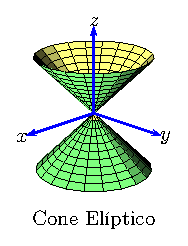
\includegraphics{cap_superficies/figs/figura_2}
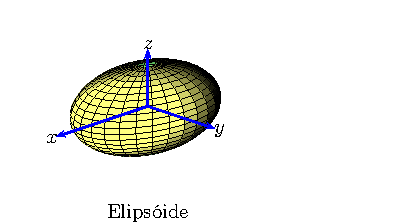
\includegraphics{cap_superficies/figs/figura_3}
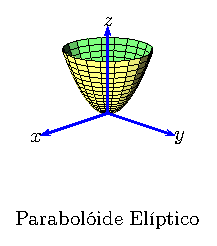
\includegraphics{cap_superficies/figs/figura_4}


\includegraphics{cap_superficies/figs/figura_5}
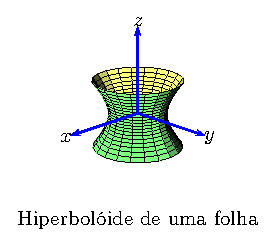
\includegraphics{cap_superficies/figs/figura_6}
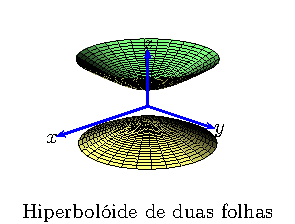
\includegraphics{cap_superficies/figs/figura_7} \caption{\label{quadricas}Quádricas}
\end{figure}

Algumas das superfícies quádricas são gráficos de funções, como é o caso dos parabolóides e outras não são, como é o caso cone elíptico. Mesmo assim, podemos definir a quádrica como a união do gráfico de duas funções. Por exemplo, o cone elíptico pode ser escrito como a união dos gráficos das funções $z=\sqrt{\frac{x^2}{a^2}+\frac{y^2}{b^2}}$ e $z=-\sqrt{\frac{x^2}{a^2}+\frac{y^2}{b^2}}$.
\end{ex}

\begin{ex}A superfície cilíndrica $x^2+y^2=9$, $0\leq z\leq 2$, pode ser escrita como a união dos gráficos das funções $x=\sqrt{9-y^2}$, $0\leq z\leq 2$ e $x=-\sqrt{9-y^2}$, $0\leq z\leq 2$.
\end{ex}

\subsection*{Exercícios}
\begin{exer}Esboce o gráfico da superfície $z=1-x^2-y^2$, $z\geq0$.
\end{exer}
\begin{exer}Esboce o gráfico da superfície $z=1-\sqrt{x^2+y^2}$, $z\geq0$.
\end{exer}
\begin{exer}Esboce o gráfico da superfície $y^2+z^2=4$, $0\leq x\geq 3$.
\end{exer}
\begin{exer}Esboce o gráfico da superfície $x+y+z=1$, no primeiro octante.
\end{exer}


%Este trabalho está licenciado sob a Licença Creative Commons Atribuição-CompartilhaIgual 3.0 Não Adaptada. Para ver uma cópia desta licença, visite https://creativecommons.org/licenses/by-sa/3.0/ ou envie uma carta para Creative Commons, PO Box 1866, Mountain View, CA 94042, USA.

\chapter{Campos vetoriais}\label{cap:campos}\index{campos vetoriais}


\chapter{Campos escalares e campos vetoriais}
 Campo é termo usado para designar funções definidas em uma porção do espaço tridimensional (ou bidimensional), isto é, funções cujo domínio $D$ é um subconjunto de $\mathbb{R}^3$ (ou $\mathbb{R}^2$). Trabalharemos com dois tipos de campos: os campos escalares e os campos vetoriais. Os campos vetoriais são funções cuja imagem é composta de vetores no $\mathbb{R}^3$, já a imagem dos campos escalares são números reais, isto é, escalares.
 
\begin{ex}\label{excampos} São exemplos de campos escalares.
\begin{itemize}
\item [a)] A função que liga a posição de um ponto dentro de uma sala à temperatura neste ponto.
\item [b)] A pressão do ar como função da posição na atmosfera.  
\item [c)] $f(x,y,z)= 100 + 20e^{-\sqrt{x^2+y^2+z^2}}$.
\item [d)] $f(x,y,z)= \vec{r} \cdot \vec{r} = x^2+y^2+z^2$, onde $\vec{r}=x\vec{i}+y\vec{j}+z\vec{k}$ .
\end{itemize}
\end{ex}   


\begin{ex}\label{excampos} São exemplos de campos vetoriais.
\begin{itemize}
\item [a)] A função que liga a posição de um ponto dentro de uma fluido à velocidade (vetor) neste ponto.
\item [b)] O campo magnéticos, elétrico, gravitacional etc.  
\item [c)] $\vec{F}(x,y,z)= x\vec{i} + z\vec{j} - y\vec{k}$.
\item [d)] $\vec{F}(x,y,z)= \vec{r}\times \vec{k}$
\end{itemize}
\end{ex}  

\section{Representação gráfica dos campos vetoriais}
Um campo vetorial é representado graficamente por um conjunto de setas partindo de pontos $(x,y,z)$ e de comprimento proporcional ao módulo de $\vec{F}(x,y,z)$ e mesma direção e sentido de $\vec{F}(x,y,z)$. O conjunto de pontos é escolhido de forma arbitrária de forma a permitir interpretar o campo.  

\begin{ex} Represente graficamente o campo vetorial $\vec{F}(x,y)=\sqrt{y}\ \!\vec{i},~~y\geq 0$.
%\begin{figure}[htp]
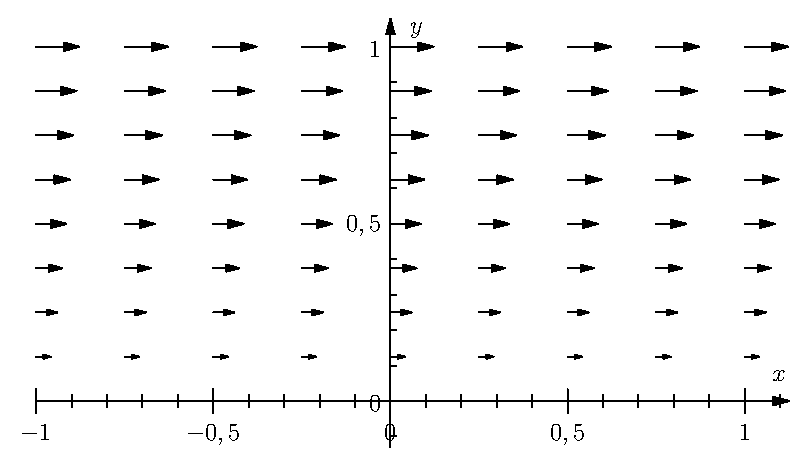
\includegraphics{cap_campos/figs/campo_exemplo_1}
%\caption{\label{campo_radial}Representação gráfica do campo $\vec{F}(x,y)=\sqrt{y}\ \!\vec{i},~~y\geq 0$.}
%\end{figure}
\end{ex}


\begin{ex} Represente graficamente o campo vetorial $\vec{F}(x,y)=x\vec{i},~~y\geq 0$.
%\begin{figure}[htp]
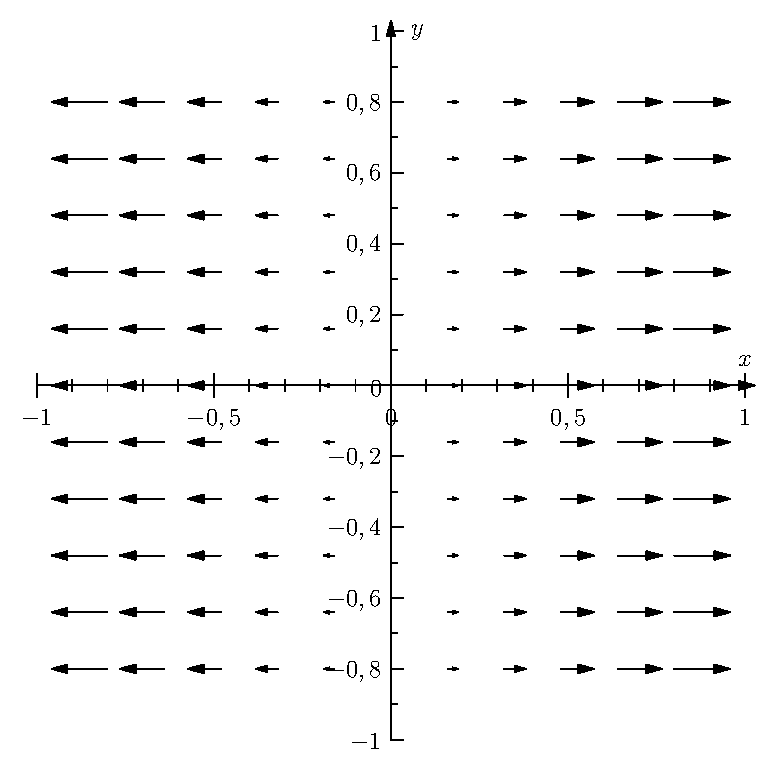
\includegraphics{cap_campos/figs/campo_exemplo_2}
%\caption{\label{campo_radial}Representação gráfica do campo $\vec{F}(x,y)=x\vec{i}$.}
%\end{figure}
\end{ex}

\begin{ex} Represente graficamente o campo vetorial $\vec{F}(x,y)=-y\vec{i}+x\vec{j}$.
%\begin{figure}[htp]
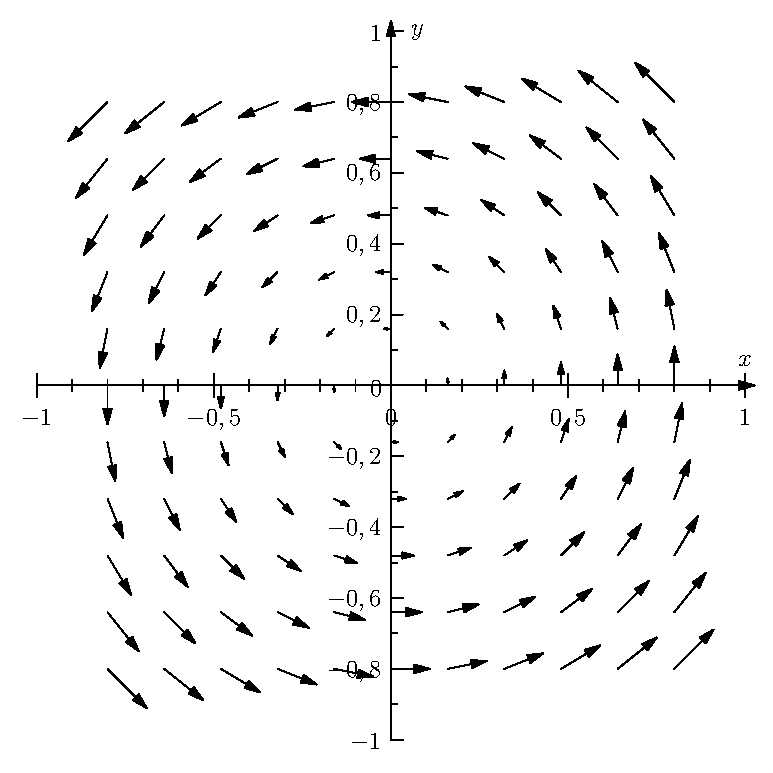
\includegraphics{cap_campos/figs/campo_exemplo_3}
%\caption{\label{campo_radial}Representação gráfica do campo $\vec{F}(x,y)=-y\vec{i}+x\vec{j}$.}
%\end{figure}
\end{ex}



\section{Cálculo com o operador $\vec{\nabla}$}
\subsection{Operador $\vec{\nabla}$}
No cálculo vetorial, o operador $\vec{\nabla}$, pronunciado nabla ou del, é um símbolo usado para denotar uma série de operadores diferenciais definidos em campos escalares e vetorias, como gradiente, divergente e rotacional. Ele é definido simbolicamente como:
\begin{equation}\label{def_del}
\vec{\nabla} \equiv \vec{i}\frac{\partial}{\partial x}+\vec{j}\frac{\partial}{\partial y}+\vec{k}\frac{\partial}{\partial z}
\end{equation}
Rigorosamente falando, o operador del não é um operador diferencial, mas um mnemônico que ajuda a lembrar de uma série de operadores diferenciais:
\begin{eqnarray*}
 \vec{\nabla}f &=& \vec{i}~\!\frac{\partial f}{\partial x}+\vec{j}~\!\frac{\partial f}{\partial y}+\vec{k}~\!\frac{\partial f}{\partial z} ~~ \text{(Gradiente)},\\
 \vec{\nabla}\cdot \vec{F} &=& \frac{\partial F_1}{\partial x}+\frac{\partial F_2}{\partial y}+\frac{\partial F_3}{\partial z} ~~ \text{(Divergente)},\\
 \vec{\nabla}\times \vec{F} &=&  \vec{i}\left(\frac{\partial F_3}{\partial y}-\frac{\partial F_2}{\partial z}\right) + \vec{j}\left(\frac{\partial F_1}{\partial z}-\frac{\partial F_3}{\partial x}\right) + \vec{k}\left(\frac{\partial F_2}{\partial x}-\frac{\partial F_1}{\partial y}\right)~~ \text{(Rotacional)}.\\
\end{eqnarray*}
$$
\left|
 \begin{array}{ccc}
 \vec{i} & \vec{j} & \vec{k} \\
 \frac{\partial}{\partial x} &\frac{\partial}{\partial y} &\frac{\partial}{\partial z} \\
F_1 & F_2 & F_3
 \end{array}
\right| 
$$
\subsection{Derivada direcional e gradiente}
\subsection{Divergente}
\subsection{Rotacional}
\section{Identidades envolvendo o operador $\vec{\nabla}$}
\begin{equation}\label{rot_grad}
\vec{\nabla}\times\vec{\nabla}f=\vec{0}
\end{equation}


\section{Campos conservativos}
\begin{defn} \label{def_campo_conservativo}\index{campo!conservativo}\index{campo!rotacional}\index{campo!gradiente}  Um campo $\vec{F}(x,y,z)$ é dito conservativo se existe um campo escalar $\varphi(x,y,z)$ tal que
$$\vec{F}(x,y,z) = \vec{\nabla}\varphi$$
Neste caso $\varphi$ é chamado de campo potencial de $$\vec{F}(x,y,z)$$
\end{defn}
\begin{obs} Campos conservativos também são conhecidos como campos grandiente ou campos irrotacionais, este último nome advém do fato que $$\vec{\nabla}\times\vec{F}(x,y,z) = \vec{\nabla}\times\vec{\nabla}\varphi=\vec{0}.$$
Esta identidade é oriunda da Equação~\ref{rot_grad}. 
 \end{obs}
\begin{ex} O campo $\vec{F}=2xy\vec{i}+x^2\vec{j}$ é conservativo por $\vec{F}=\vec{\nabla}\left(x^2y\right)$.
 \end{ex}

\begin{teo} Seja $\vec{F}:\mathbb{R}^3\to\mathbb{R}^3$ um campo vetorial contínuo e $\vec{\nabla}\times \vec{F}=\vec{0}$, então $\vec{F}$ é conservativo.
 \end{teo}
\begin{proof} Como $\vec{\nabla}\times \vec{F}=\vec{0}$, temos:
\begin{eqnarray}
 \frac{\partial F_3}{\partial y} &=&\frac{\partial F_2}{\partial z}\label{rot_zero_x},\\
 \frac{\partial F_1}{\partial z} &=&\frac{\partial F_3}{\partial x}\label{rot_zero_y},\\
 \frac{\partial F_3}{\partial x} &=&\frac{\partial F_1}{\partial y}\label{rot_zero_z}.
\end{eqnarray}
Defina, agora, a função $\varphi:\mathbb{R}^3\to\mathbb{R}$ dada por
$$\varphi(x,y,z)=\int_0^xF_1(s,y,z) + \int_0^yF_2(0,s,z)+\int_0^zF_3(0,0,s).$$
Basta provar que $\vec{\nabla}\varphi(x,y,z)=\vec{F}$, isto é
\begin{eqnarray}
 \frac{\partial \varphi}{\partial z} &=&F_1,\label{rot_zero_der_x}\\
 \frac{\partial \varphi}{\partial y} &=&F_2,\label{rot_zero_der_y}\\
 \frac{\partial \varphi}{\partial z} &=&F_3\label{rot_zero_der_z}.
\end{eqnarray}
A primeira desigualdade advém diretamente do teorema fundamental do cálculo. Para obter a segunda desigualdade, derivamos o potencial em relação a $y$:
\begin{eqnarray*}
\frac{\partial }{\partial y}\varphi(x,y,z)&=&\int\int 0^x \frac{\partial }{\partial y}F_1(s,y,z)ds+ F_2(0,y,z)\\
&=&\int_0^x \frac{\partial }{\partial s}F_2(s,y,z)ds+ F_2(0,y,z)\\
&=&\left(F_2(x,y,z)-F_2(0,y,z)\right)+ F_2(0,y,z) = F_2(x,y,z)
\end{eqnarray*}
Onde usamos a Identidade~\ref{rot_zero_y}.

Finalmente, para obter a terceira desigualdade, derivamos o potencial em relação a $z$:
\begin{eqnarray*}
\frac{\partial }{\partial z}\varphi(x,y,z)&=&\int_0^x \frac{\partial }{\partial z}F_1(s,y,z)ds + \int_0^y \frac{\partial }{\partial z}F_2(0,s,z)ds+F_3(0,0,z)\\
&=&\int_0^x \frac{\partial }{\partial s}F_3(s,y,z)ds + \int_0^ \frac{\partial }{\partial s}F_3(0,s,z)ds+F_3(0,0,z)\\
&=&\int_0^x \left(F_3(x,y,z)-F_3(0,y,z)\right) + \left(F_3(0,y,z)-F_3(0,0,z)\right)+F_3(0,0,z)\\
&=&F_3(x,y,z)\\
\end{eqnarray*}
  Onde usamos as Idendidade~\ref{rot_zero_x} e \ref{rot_zero_z}.
\end{proof}

 
 

\section{Campos radiais e potenciais centrais}
Campos radiais vetoriais \index{campos radiais} são campos da forma $\vec{F}=f(r) \hat{r}$, isto é campos vetoriais cujo módulo depende apenas da distância até a origem, isto é, de $r=\|\vec{r}\|=\sqrt{x^2+y^2+z^2}$ e cuja direção é sempre paralela ao vetor posição, $\vec{r}$.
\begin{ex} Represente graficamente o campo vetorial $\vec{F}=\vec{r}$ no plano $xy$.
%\begin{figure}[htp]
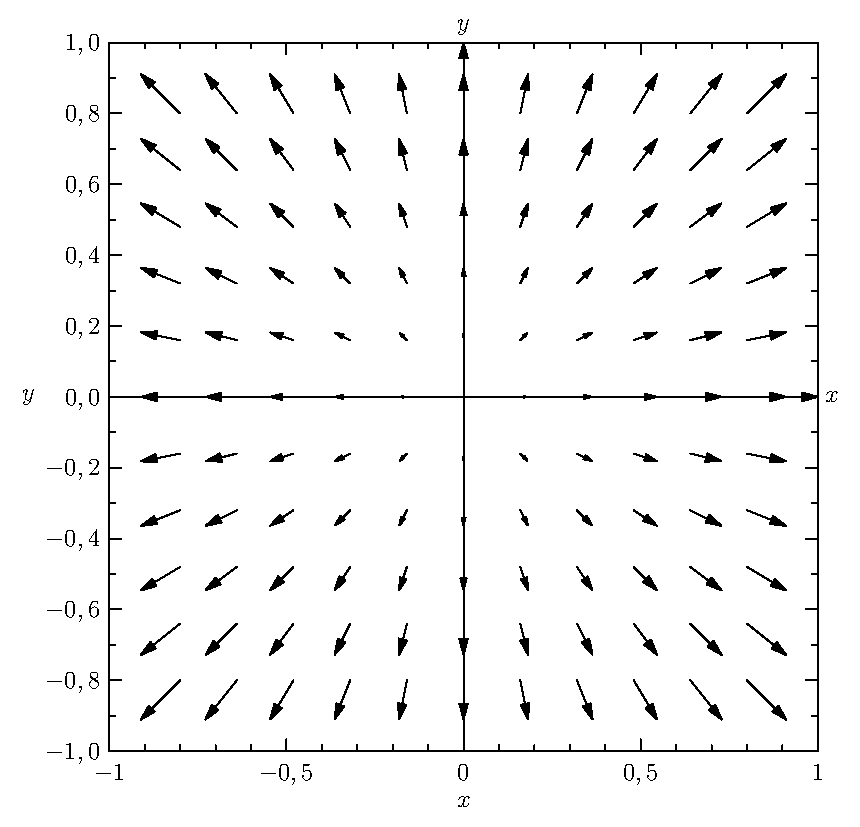
\includegraphics{cap_campos/figs/campo_radial}
%\caption{\label{campo_radial}Representação gráfica do campo $\vec{F}=\vec{r}$}
%\end{figure}
\end{ex}





\construirSec

\subsection*{Exercícios resolvidos}

\construirExeresol

\begin{exeresol}
  Um exercício.
\end{exeresol}
\begin{resol}
  Resolução do exercício.
\end{resol}

\subsection*{Exercícios}

\construirExer

\begin{exer}
  Um exercício.
\end{exer}
\begin{resp}
  Resposta curta do exercício.
\end{resp}

\section{Exercícios finais}

\construirExer

\begin{exer}
  Um exercício.
\end{exer}
\begin{resp}
  Resposta curta do exercício.
\end{resp}

 %+Diferenciação
%Este trabalho está licenciado sob a Licença Creative Commons Atribuição-CompartilhaIgual 3.0 Não Adaptada. Para ver uma cópia desta licença, visite https://creativecommons.org/licenses/by-sa/3.0/ ou envie uma carta para Creative Commons, PO Box 1866, Mountain View, CA 94042, USA.
% !TEX root = ../main.tex

\chapter{Integral de Linha}
  Neste capítulo, estudamos a integral de linha\index{integral de linha} e teoremas relacionados.
\section{A integral de linha para um campo escalar}
Para um campo escalar $f:D\to\mathbb{R}$, $D\subset \mathbb{R}^3$, a integral de linha ao longo de uma curva suave por partes é definida por
$$
\int_{\mathcal{C}} f(\vec{r})\, ds = \int_a^b f\left(\vec{r}(t)\right) \left|\vec{r}'(t)\right| \, dt,
$$
onde $\vec{r}$ é uma parametrização para $C$ tal que $\vec{r}(a)$ e $\vec{r}(b)$ são os pontos iniciais e finais da curva.
\section{A integral de linha para um campo vetorial}
Para um campo vetorial $\vec{F}:D\to\mathbb{R}^3$, $D\subset \mathbb{R}^3$, a integral de linha ao longo de uma curva suave por partes $C$ é definida por
$$
\int_C \vec{F}(\vec{r})\cdot\,d\vec{r} = \int_a^b \vec{F}(\vec{r}(t))\cdot\vec{r}'(t)\,dt
$$
onde $\vec{r}$ é uma parametrização para $C$ tal que $\vec{r}(a)$ e $\vec{r}(b)$ são os pontos iniciais e finais da curva, que está no sentido $\vec{r}(a)\to \vec{r}(b)$.


\subsection*{Exercícios}
\begin{exer}Calcule a integral de linha $\int_C\vec{F}\cdot d\vec{r}$ para cada campo e curva dados.
\begin{itemize}
 \item[a)] $\vec{F}=(x+2y)\vec{i}+(x-y)\vec{j},$ e $C$: $x=\cos(t)$, $y=4\sin(t)$, $0\leq t\leq \frac{\pi}{4}$.
 \item[b)] $\vec{F}=(x^2+y^2)\vec{i}-x\vec{j},$ e $C$: arco da circunferência $x^2+y^2=1$ limitado ao primeiro quadrante e orientado no sentido $(1,0)$ a $(0,1)$.
 \end{itemize}
\end{exer}
\begin{resp}
 \begin{itemize}
  \item[a)] $1-\pi$.
  \item[b)] $-1-\frac{\pi}{4}$.
 \end{itemize}
\end{resp}
\begin{exer}
 Calcule o trabalho ao se deslocar uma partícula no campo de força $\vec{F}=3x^2\vec{i}+(2xz-y)\vec{j}+z\vec{k}$ ao longo.
 \begin{itemize}
  \item[a)] da reta que liga $(0,0,0)$ a $(2,1,3)$. 
  \item[b)] da curva $x=2t^2$, $y=t$, $z=4t^2-t$ de $t=0$ até $t=1$.
  \item[c)] da curva definida por $x=4y$, $3x^3=8z$, de $x=0$ até $x=2$.
 \end{itemize}
 \end{exer}
\begin{resp}
 \begin{itemize}
  \item[a)] $16$.
  \item[b)] $14.2$.
  \item[c)] $16$.
 \end{itemize}
\end{resp}
\begin{exer}
 Dado $\vec{F}=(x-y)\vec{i}+(x+y)\vec{j}$, calcule $\oint\vec{F}\cdot d\vec{r}$ ao longo da curva $C$ dada pela união da curva $y=x^2$, desde o ponto $(0,0)$ até $(1,1)$, da curva $y=\sqrt{x}$, desde o ponto $(1,1)$ até $(0,0)$.
\end{exer}
\begin{resp}
 $\frac{2}{3}$.
\end{resp}






\section{O Teorema Fundamental para Integral de Linha}
\begin{teo}\index{teorema fundamental para integral de linha}Seja $\vec{F}$ um campo vetorial definido numa região $R$ do espaço e $P_0(x_0,y_0,z_0)$ e $P_1(x,y,z)$ dois pontos em $R$. Se $\vec{F}$ é conservativo \index{campo!conservativo}, isto é, $\vec{F}=\vec{\nabla}\varphi$ para algum potencial $\varphi$, então
\begin{equation}\label{TeoFundCalculo}
\int_C\vec{F}\cdot d \vec{r} =\varphi(x,y,z)-\varphi(x_0,y_0,z_0),
\end{equation}
para qualquer curva $C$ suave por partes em $R$ com início em $P_0$ e extremidade em $P$.

Reciprocamente, se
$$
\int_C\vec{F}\cdot d \vec{r}
$$
é independente da curva que começa em $P_0$ e termina em $P_1$, então o campo é conservativo.
\end{teo}
\begin{proof}
Sem perda de generalidade, suponha $C$ uma curva suave parametrizada por $\vec{r}(t)=x(t)\vec{i}+y(t)\vec{j}+z(t)\vec{k}$, $t_0\leq t\leq t_1$, com início em $\vec{r}(t_0)=P_0$ e fim em $\vec{r}(t_1)=P$. Então, supondo que $\vec{F}$ é conservativo, isto é, $\vec{F}=\vec{\nabla}\varphi$, temos
\begin{eqnarray*}
\int_C\vec{F}\cdot d \vec{r} &=& \int_C\vec{\nabla}\varphi\cdot d \vec{r}\\
&=& \int_{t_0}^{t_1}\vec{\nabla}\varphi\cdot \vec{r}'(t)dt\\
&=& \int_{t_0}^{t_1}\left(\frac{\partial\varphi}{\partial x}\vec{i}+\frac{\partial\varphi}{\partial y}\vec{j}+\frac{\partial\varphi}{\partial z}\vec{k}\right)\cdot \left(\frac{\partial x}{\partial t}\vec{i}+\frac{\partial y}{\partial t}\vec{j}+\frac{\partial z}{\partial t}\vec{k}\right) dt\\
&=& \int_{t_0}^{t_1}\left(\frac{\partial\varphi}{\partial x}\frac{\partial x}{\partial t}+\frac{\partial\varphi}{\partial y}\frac{\partial y}{\partial t}+\frac{\partial\varphi}{\partial z}\frac{\partial z}{\partial t}\right) dt.
\end{eqnarray*}
Usando a regra da cadeia, temos que o termo
$$
\frac{D\varphi}{Dt}=\frac{\partial\varphi}{\partial x}\frac{\partial x}{\partial t}+\frac{\partial\varphi}{\partial y}\frac{\partial y}{\partial t}+\frac{\partial\varphi}{\partial z}\frac{\partial z}{\partial t}
$$
é a derivada total de $\varphi$ com respeito a $t$. Logo, pelo Teorema Fundamental do Cálculo, temos:
\begin{eqnarray*}
\int_C\vec{F}\cdot d \vec{r} &=&  \int_{t_0}^{t_1}\frac{D\varphi}{Dt} dt\\
&=& \varphi(x(t_1),y(t_1),z(t_1))- \varphi(x(t_0),y(t_0),z(t_0))\\
&=& \varphi(x,y,z)- \varphi(x_0,y_0,z_0).
\end{eqnarray*}
Reciprocamente, dado que a expressão \eqref{TeoFundCalculo} é válida para qualquer curva $C$ que liga dois pontos na região, definimos a função
$$
\varphi(x,y,z)=\int_C \vec{F}\cdot d\vec{r}=\int_{P_0}^{P_1} \vec{F}\cdot d\vec{r}=\int_{(x_0,y_0,z_0)}^{(x,y,z)} \vec{F}\cdot d\vec{r},
$$
onde $C$ é uma curva qualquer que começa em $P_0$ e termina em $P$. Mostraremos que $\phi$ é o potencial do campo $\vec{F}=F_1\vec{i}+F_2\vec{j}+F_3\vec{k}$, ou seja, $\vec{F}=\vec{\nabla}\varphi$. De fato, observe que
\begin{eqnarray*}
\varphi(x+\Delta x,y,z)-\varphi(x,y,z)&=&\int_{(x_0,y_0,z_0)}^{(x+\Delta x,y,z)} \vec{F}\cdot d\vec{r}-\int_{(x_0,y_0,z_0)}^{(x,y,z)} \vec{F}\cdot d\vec{r}\\
&=&\int_{(x_0,y_0,z_0)}^{(x+\Delta x,y,z)} \vec{F}\cdot d\vec{r}+\int^{(x_0,y_0,z_0)}_{(x,y,z)} \vec{F}\cdot d\vec{r}\\
&=&\int_{(x,y,z)}^{(x+\Delta x,y,z)} \vec{F}\cdot d\vec{r}.
\end{eqnarray*}
Parametrizando um caminho reto entre $(x,y,z)$ e $(x+\Delta x,y,z)$ por $\vec{r}=t\vec{i}+y\vec{j}+z\vec{k}$, $x\leq t\leq \Delta x$, temos:
\begin{eqnarray*}
\varphi(x+\Delta x,y,z)-\varphi(x,y,z)&=&\int_x^{x+\Delta x} \vec{F}\cdot \vec{r}' dt \\
&=&\int_x^{x+\Delta x} \left(F_1\vec{i}+F_2\vec{j}+F_3\vec{k}\right)\cdot \vec{i} dt\\
&=&\int_x^{x+\Delta x} F_1 (t,y,z) dt .
\end{eqnarray*}
Logo, pelo teorema do valor médio,
\begin{eqnarray*}
\frac{\varphi(x+\Delta x,y,z)-\varphi(x,y,z)}{\Delta x}&=& \frac{1}{\Delta x}\int_x^{x+\Delta x} F_1 (t,y,z) dt\\
&=& \frac{1}{\Delta x}  F_1 (\xi,y,z) , \qquad x\leq \xi\leq x+\Delta x.
\end{eqnarray*}
Portanto,
\begin{eqnarray*}
\frac{\partial \varphi}{\partial x}&=&\lim_{\Delta x\to 0}\frac{\varphi(x+\Delta x,y,z)-\varphi(x,y,z)}{\Delta x}\\
&=&\lim_{\Delta x\to 0} \frac{1}{\Delta x}  F_1 (\xi,y,z)\\
&=&F_1 (x,y,z).
\end{eqnarray*}
Analogamente, podemos demonstrar que
$$
\frac{\partial \varphi}{\partial y}=F_2(x,y,z) \qquad \text{e}\qquad \frac{\partial \varphi}{\partial z}=F_3(x,y,z),
$$
ou seja, $\vec{F}=\vec{\nabla}\varphi.$
\end{proof}

\subsection*{Exercícios}
\begin{exer}Calcule o trabalho realizado pela força conservativa $\vec{F}=xy^2\vec{i}+x^2y\vec{j}$ ao deslocar uma partícula desde $P_0(1,1)$ até $P_1(0,0)$.
\end{exer}
\begin{resp}
 $-\frac{1}{2}$.
\end{resp}


\section{Relação entre campos irrotacionais e conservativos}
\begin{teo}Seja $\vec{F}$ um campo vetorial definido numa região $R$ do espaço. Então $\vec{F}$ é conservativo \index{campo!conservativo}, isto é, $\vec{F}=\vec{\nabla}\varphi$ para algum potencial $\varphi$, se e somente se $\vec{F}$ é irrotacional, \index{campo!irrotacional}, isto é, $\vec{\nabla}\times \vec{F}=\vec{0}$.
\end{teo}
\begin{proof}Se $\vec{F}$ é conservativo, isto é, $\vec{F}=\vec{\nabla}\varphi$, então pelo item 8 da tabela de indentidades~\ref{tab_identidades_del}, $$\vec{\nabla}\times \vec{F}=\vec{\nabla}\times \vec{\nabla}\varphi=\vec{0}.$$
Reciprocamente, dado $\vec{F}=F_1\vec{i}+F_2\vec{j}+F_3\vec{k}$ com 
$$
\vec{\nabla }\times \vec{F}=\left| \begin{array}{ccc}
 \vec{i} & \vec{j} & \vec{k} \\
 \frac{\partial}{\partial x} &\frac{\partial}{\partial y} &\frac{\partial}{\partial z} \\
F_1 & F_2 & F_3
 \end{array}\right|=\vec{0},
 $$ 
temos
\begin{equation}\label{rot_zero_eq1}
 \frac{\partial F_3}{\partial y}=\frac{\partial F_2}{\partial z},
\end{equation}
\begin{equation}\label{rot_zero_eq2}
 \frac{\partial F_1}{\partial z}=\frac{\partial F_3}{\partial x}
\end{equation}
e
\begin{equation}\label{rot_zero_eq3}
 \frac{\partial F_2}{\partial x}=\frac{\partial F_1}{\partial y}.
\end{equation}
Agora, defina
\begin{equation}\label{def_pot_campo_conser}
\varphi(x,y,z)=\int_C \vec{F}\cdot d\vec{r},
\end{equation}
onde $C$ é a curva que liga os pontos $(x_0,y_0,z_0)$ ao ponto $(x,y,z)$ através das arestas do paralelepípedo de vértices $(x_0,y_0,z_0)$, $(x,y_0,z_0)$, $(x_0,y,z_0)$, $(x,y,z_0)$, $(x_0,y_0,z)$, $(x,y_0,z)$, $(x_0,y,z)$ e $(x,y,z)$. Isto é, $C$ pode ser escrito com a união de três segmentos de retas, $C=C_1 \cup C_2\cup C_3$, com as seguintes parametrizações: 
$$
C_1: \vec{r}_1(t)=t\vec{i}+y_0\vec{j}+z_0\vec{k},\qquad x_0\leq t\leq x,
$$ 
$$
C_2: \vec{r}_2(t)=x\vec{i}+t\vec{j}+z_0\vec{k},\qquad y_0\leq t\leq y
$$ 
e
$$
C_3: \vec{r}_3(t)=x\vec{i}+y\vec{j}+t\vec{k},\qquad z_0\leq t\leq z.
$$ 
Mostraremos que $\varphi$ é um potencial para o campo $\vec{F}$, isto é, $\vec{F}=\vec{\nabla}\varphi$. De fato, da equação \eqref{def_pot_campo_conser}, usamos as parametrizações das curvas $C_1$, $C_2$ e $C_3$ para obter
\begin{eqnarray}
\nonumber \varphi(x,y,z)&=&\int_{C_1} \vec{F}\cdot d\vec{r}+\int_{C_2} \vec{F}\cdot d\vec{r}+\int_{C_3} \vec{F}\cdot d\vec{r}\\
\nonumber&=&\int_{x_0}^x \vec{F}\cdot \vec{r}'_1(t)dt+ \int_{y_0}^y \vec{F}\cdot \vec{r}'_2(t)dt+\int_{z_0}^z \vec{F}\cdot \vec{r}'_3(t)dt\\
&=&\int_{x_0}^x F_1(t,y_0,z_0) d t+ \int_{y_0}^y F_2(x,t,z_0)dt+\int_{z_0}^z F_3(x,y,t)dt.\label{def_pot_campo_conser_calculado}
\end{eqnarray}
Pelo Teorema Fundamental do Cálculo, derivamos a expressão \eqref{def_pot_campo_conser_calculado} em $z$ e obtemos a última componente do campo:
\begin{equation}\label{gradiente_3_comp}
\frac{\partial \varphi}{\partial z}=F_3(x,y,z). 
\end{equation}
Agora, derivamos a expressão \eqref{def_pot_campo_conser_calculado} em $y$
\begin{eqnarray*}
\frac{\partial \varphi}{\partial y}&=&F_2(x,y,z_0)+\frac{\partial}{\partial y}\int_{z_0}^z F_3(x,y,t)dt\\
&=&F_2(x,y,z_0)+\int_{z_0}^z \frac{\partial F_3(x,y,t)}{\partial y}dt\\ 
&=&F_2(x,y,z_0)+\int_{z_0}^z \frac{\partial F_2(x,y,t)}{\partial z}dt. 
\end{eqnarray*}
onde usamos a expressão \eqref{rot_zero_eq1} na última passagem. Assim, usamos o Teorema Fundamental do Cálculo para obter
\begin{equation}\label{gradiente_2_comp}
\frac{\partial \varphi}{\partial y}=F_2(x,y,z_0)+F_2(x,y,z)-F_2(x,y,z_0)=F_2(x,y,z). 
\end{equation}
Finalmente, derivamos a expressão \eqref{def_pot_campo_conser_calculado} com respeito a $x$:
\begin{eqnarray*}
\frac{\partial \varphi}{\partial x}&=&F_1(x,y_0,z_0) d t+ \frac{\partial}{\partial x}\int_{y_0}^y F_2(x,t,z_0)dt+ \frac{\partial}{\partial x}\int_{z_0}^z F_3(x,y,t)dt\\
&=&F_1(x,y_0,z_0) d t+ \int_{y_0}^y \frac{\partial F_2(x,t,z_0)}{\partial x}dt+ \int_{z_0}^z \frac{\partial F_3(x,y,t)}{\partial x}dt\\
&=&F_1(x,y_0,z_0) d t+ \int_{y_0}^y \frac{\partial F_1(x,t,z_0)}{\partial y}dt+ \int_{z_0}^z \frac{\partial F_1(x,y,t)}{\partial z}dt,
\end{eqnarray*}
onde usamos as expressões \eqref{rot_zero_eq2} e \eqref{rot_zero_eq3} na última passagem. Assim, usamos o Teorema Fundamental do Cálculo para concluir que
\begin{eqnarray}
\nonumber \frac{\partial \varphi}{\partial x}&=&F_1(x,y_0,z_0)+F_1(x,y,z_0)-F_1(x,y_0,z_0)+F_1(x,y,z)-F_1(x,y,z_0)\\
&=&F_1(x,y,z)\label{gradiente_1_comp}
\end{eqnarray}

Portanto, das expressões \eqref{gradiente_1_comp}, \eqref{gradiente_2_comp} e \eqref{gradiente_3_comp}, concluímos que $\vec{F}=\vec{\nabla}\varphi$, ou seja, $\vec{F}$ é um campo conservativo.
\end{proof}

\subsection*{Exercícios resolvidos}
\begin{exeresol}
  Dado o campo vetorial $\vec{F}(x,y,z) = 2xy^3+(1+3x^2y^2)\vec{j}$.
  \begin{itemize}
  \item[a)] Mostre que o campo é irrotacional.
  \item[b)] Encontre uma função potencial $\varphi(x,y,z)$.
  \item[c)] Calcule o trabalho $W:=\int_C \vec{F}\cdot d\vec{r}$ ao longo de uma curva que liga o ponto $(1,4,0)$ até o ponto $(3,1,0)$.
  \item[d)] Trace algumas curvas equipotenciais de $\varphi(x,y,z)$.
  \end{itemize}
\end{exeresol}
\begin{resol}
  Para o item a), basta calcular o rotacional:
  \begin{eqnarray*}
  \vec{\nabla}\times \vec{F} &=& \left|
  \begin{array}{ccc}
  \vec{i} & \vec{j} & \vec{k} \\
  \frac{\partial}{\partial x} & \frac{\partial}{\partial y} & \frac{\partial}{\partial z}\\
  2xy^3 & 1+3x^2y^2 & 0
  \end{array}
  \right| \\
  &=& \left(0-0\right)\vec{i} + \left(0-0\right)\vec{j} + \left(6xy^2-6xy^2\right)\vec{k}\\
  &=& \vec{0}
  \end{eqnarray*}
A função potencial $\varphi$ deve satisfazer $\vec{\nabla}\varphi=\vec{F}$, isto é:
\begin{eqnarray*}
\frac{\partial \varphi}{\partial x} &=& 2xy^3 \\
\frac{\partial \varphi}{\partial y} &=& 1+x^2y^2 \\
\frac{\partial \varphi}{\partial z} &=& 0
\end{eqnarray*}
Da primeira equação, temos $\varphi(x,y,z)= x^2y^3+C(y,z)$. Diferenciando esta expressão substituindo na segunda condição, temos:
\begin{eqnarray*}
\frac{\partial }{\partial y}(x^2y^3+C(y,z)) &=& 1+x^2y^2.
\end{eqnarray*}
Isso implica $C_y(y,z)=1$, isto é, $C(y,z) = y+D(z)$. Da última expressão vemos que $D'(z)=0$ e portanto:
$$\varphi(x,y,z)=x^2y^3+y+E.$$
Para o item c), basta aplicar o teorema das integrais de linha:
\begin{eqnarray*}
W &=& \int_C \vec{F}\cdot d\vec{r} = \varphi(3,1,0)- \varphi(1,4,0)\\
  &=& (9+1+E) - (64+4+E) = -58.
\end{eqnarray*}
\end{resol}

\subsection*{Exercícios}
\begin{exer}Determine se o campo $\vec{F}$ é conservativo. Se for, encontre a função potencial $\phi$.
 \begin{itemize}
  \item[a)] $\vec{F}=x\vec{i}+y\vec{j}$.
  \item[b)] $\vec{F}=x^2y\vec{i}+5xy^2\vec{j}$.
  \item[c)] $\vec{F}=(\cos(y)+y\cos(x))\vec{i}+(\sin(x)-x\sin(y))\vec{j}$.
  \item[d)] $\vec{F}=yz\vec{i}+xz\vec{j}+(xy+3z^2)\vec{k}$.
 \end{itemize}
 \end{exer}
\begin{resp}
  \begin{itemize}
  \item[a)] $\phi=\frac{1}{2}\left(x^2+y^2\right)+C$.
  \item[b)] Não é conservativo.
  \item[c)] $\phi=x\cos(y)+y\sin(x)+C$.
  \item[d)] $\phi=xyz+z^3+C$.
 \end{itemize}
\end{resp}

\begin{exer}
 Calcule $\int_C\vec{F}\cdot d\vec{r}$, para $\vec{F}=(e^y+ye^x)\vec{i}+(xe^y+e^x)\vec{j}$ e $C$ é a curva dada por $\vec{r}=\sin\left(\frac{\pi}{2}t\right)\vec{i}+(\ln(t))\vec{j}$, $1\leq t\leq 2$. 
 
 {\it (Sugestão: Determine primeiro se $\vec{F}$ é conservativo).}
\end{exer}
\begin{resp}
 $-1+\ln(2)$.
\end{resp}

\begin{exer}Se $\vec{A}=(4xy-3x^2z^2)\vec{i}+2x^2\vec{j}-2x^3z\vec{k}$, prove que $\int_C\vec{A}\cdot d\vec{r}$ é independente da curva que liga dois pontos dados. 
\end{exer}
\begin{exer}Seja $\vec{E}=r\vec{r}$.
 \begin{itemize}
  \item[a)] Prove que existe um potencial $\phi$ tal que $\vec{E}=\vec{\nabla}\phi$.
  \item[b)] Calcule $\phi$.
  \item[c)] Calcule o valor de $\oint_C\vec{E}\cdot d\vec{r}$ para $C$ a circunferência de raio unitário no plano $xy$ orientada no sentido horário. É possível conhecer o valor de $\oint_C\vec{E}\cdot d\vec{r}$ onde $C$ é uma curva fechada qualquer? \end{itemize}
\end{exer}

 \begin{resp}
 \begin{itemize}
  \item[b)] $\phi=\frac{r^3}{3}+C$.
  \item[c)] $0$
 \end{itemize}
 \end{resp}

 \begin{exer}
  Calcule o trabalho para se deslocar uma partícula nos campos de força conservativa dados por:
  \begin{itemize}
   \item[a)] $\vec{F}=-k\vec{r}$ (Lei de Hooke).
   \item[b)] $\vec{F}=\frac{1}{r^3}\vec{r}$ (Lei do inverso do quadrado).
  \end{itemize}
 \end{exer}
\begin{resp}
   \begin{itemize}
   \item[a)] $\phi=-\frac{k r^2}{2}+C$.
   \item[b)] $\phi=-\frac{1}{r}+C$.
  \end{itemize}
\end{resp}



\section{O Teorema de Green}
\begin{teo}
 Seja $C$ uma curva simples, fechada e derivável, $D$ a região do plano delimitada por $C$, e $P$ e $Q$ duas funções reais de variável real com derivadas parciais contínua numa região contendo $D$, então:

$$\int_{C} (P dx + Q dy) = \iint_{D} \left(\frac{\partial Q}{\partial x} - \frac{\partial P}{\partial
y}\right) dA.
$$
Em termo de notação, também se costuma usar $\oint_C$ para enfatiza que o caminho $C$ é fechado. Nesse caso, supondo $\vec{F}=P\vec{i}+Q\vec{j}$, podemos escrever o teorema da forma
$$
\oint_C  \vec{F} \cdot d\vec{r}=\iint_{D} \left(\frac{\partial Q}{\partial x} - \frac{\partial P}{\partial
y}\right) dA.
$$
\end{teo}


 %+Integral de Linha e teoremas
%Este trabalho está licenciado sob a Licença Creative Commons Atribuição-CompartilhaIgual 3.0 Não Adaptada. Para ver uma cópia desta licença, visite https://creativecommons.org/licenses/by-sa/3.0/ ou envie uma carta para Creative Commons, PO Box 1866, Mountain View, CA 94042, USA.
% !TEX root = ../main.tex
\chapter{Integral de Superfície}
  Neste capítulo, estudamos a integral de superfície\index{integral de superfície} e teoremas relacionados.
\section{Definição de integral de superfície para um campo escalar}

Seja $h: \mathbb{R}^3\to \mathbb{R}$, $h= h(x,y,z)$, um campo escalar definido em todos os pontos de uma superfície regular $S$. Assumimos que $\vec{r}(u,v)=x(u,v)\vec{i}+y(u,v)\vec{j}+z(u,v)\vec{k}$, $(u,v)\in R \subset \mathbb{R}^2$ seja uma parametrização para $S$. A integral de superfície de $h$ sobre $S$ é definida por:
\begin{equation}\label{definicao_int_sup_esc}
\iint_S h d S = \iint_R h(x(u,v),y(u,v),z(u,v)) \|\vec{r}_u\times \vec{r}_v\|d udv, 
\end{equation}
onde $dS$ é o elemento infinitesimal de área sobre a superfície.


\begin{ex}\label{ex_esfera_int_sup}Considere a esfera de raio $a$ 
$$
\vec{r}=a\sin(u)\cos(v)\vec{i}+a\sin(u)\sin(v)\vec{j}+a\cos(u)\vec{k},~~ a>0, ~ 0\leq u< \pi, ~ 0\leq v< 2\pi
$$
e o campo $h(x,y,z)=1$. Vamos calcular a área da esfera dada por $\iint_S h d S $. Começamos com as derivadas parciais de $\vec{r}$, dadas por
$$
\vec{r}_u=a\cos(u)\cos(v)\vec{i}+a\cos(u)\sin(v)\vec{j}-a\sin(u)\vec{k}
$$
e
$$
\vec{r}_v=-a\sin(u)\sin(v)\vec{i}+a\sin(u)\cos(v)\vec{j}.
$$
Então, temos
\begin{eqnarray}
\label{prod_vet_ru_rv}  \vec{r}_u\times\vec{r}_v&=&\left|
 \begin{array}{ccc}
 \vec{i} & \vec{j} & \vec{k} \\
  a\cos(u)\cos(v)&a\cos(u)\sin(v)&-a\sin(u) \\
-a\sin(u)\sin(v)&a\sin(u)\cos(v)&0
 \end{array}
\right|\\
\nonumber &=& a^2\sin^2(u)\cos(v)\vec{i}+ a^2\sin^2(u)\sin(v)\vec{j}\\\nonumber&+&(a^2\cos(u)\sin(u)\cos^2(v)+ a^2\cos(u)\sin(u)\sin^2(v))\vec{k}\\
\nonumber &=& a^2\sin^2(u)\cos(v)\vec{i}+ a^2\sin^2(u)\sin(v)\vec{j}+a^2\cos(u)\sin(u)\vec{k}.
\end{eqnarray}
e
\begin{eqnarray*}
\|  \vec{r}_u\times\vec{r}_v\|&=&a^2\sqrt{ \sin^4(u)(\cos^2(v)+ \sin^2(v))+\cos^2(u)\sin^2(u)}\\
&=&a^2\sqrt{ \sin^4(u)+\cos^2(u)\sin^2(u)}\\
&=&a^2\sin(u)\sqrt{ \sin^2(u)+\cos^2(u)}\\
&=&a^2\sin(u).
\end{eqnarray*}
onde usamos que $0\leq \sin(u)\leq 1$, visto que $0\leq u\leq \pi$. Portanto,
\begin{eqnarray*}
\iint_S h d S &=& \iint_R h(x(u,v),y(u,v),z(u,v)) \|\vec{r}_u\times \vec{r}_v\|d udv \\
&=& \int_0^{2\pi}\int_0^{\pi} a^2\sin(u) d udv \\
&=&2\pi a^2 \left[ -\cos(u) \right]_0^{\pi}\\
&=&4\pi a^2.
\end{eqnarray*}

\end{ex}
\subsection{Superfície definida como função de duas variáveis}
Nessa seção, vamos calcular a versão particular da definição \eqref{definicao_int_sup_esc} quando a superfície é definida como função de duas variáveis, isto é, $z=f(x,y)$ ou $y=f(x,z)$ ou ainda $x=f(y,z)$. Considere o caso onde a superfície $S$ é dado pela função $f:D\subset\mathbb{R}$, $D\subset \mathbb{R}^2$, $z=f(x,y)$ (os outros dois casos são análogos). Uma parametrização para a superfície $S$ é
$$
\vec{r}(x,y)= x\vec{i}+ y\vec{j}+ f(x,y)\vec{k},
$$
Calculamos as derivadas $\vec{r}_x=\vec{i}+ f_x\vec{k},$ e $\vec{r}_y=\vec{j}+ f_y\vec{k}$ e fazemos
$$
  \vec{r}_x\times\vec{r}_y=\left|
 \begin{array}{ccc}
 \vec{i} & \vec{j} & \vec{k} \\
  1 &0 & f_x \\
0 &  1 & f_y
 \end{array}
\right|\\= f_x\vec{i}+ f_y\vec{j}+\vec{k}.
$$
Agora, definimos $G$ tal que a superfície seja reescrita como $G(x,y,z)=0$, isto é, $G(x,y,z)=z-f(x,y)$ e observamos que
\begin{equation}\label{normal_grad_G_0}
   \vec{r}_x\times\vec{r}_y=\vec{ \nabla} G.
\end{equation}
Analogamente, em qualquer dos outros dois casos $y=f(x,z)$ ou $x=f(y,z)$, definimos $G$ tal que a superfície seja reescrita como $G(x,y,z)=0$ e a expressão \eqref{normal_grad_G_0} continua válida, isto é,
\begin{equation*}\label{normal_grad_G_0_2}
   \vec{r}_x\times\vec{r}_z=\vec{ \nabla} G\qquad \text{ou} \qquad    \vec{r}_y\times\vec{r}_z=\vec{ \nabla} G.
\end{equation*}
Portanto, a versão da definição \eqref{definicao_int_sup_esc} para o caso onde a superfície é definida por uma função de duas variáveis $f$ é dada por
\begin{equation}\label{definicao_int_sup_esc_par}
\iint_S h d S=  \iint_R h\| \vec{\nabla}G\| dA,
\end{equation}
onde $R$ é o domínio de $h$ e $h$ deve estar sobre os pontos da superfície.

\begin{ex}Vamos calcular novamente a integral de supefície do exemplo \ref{ex_esfera_int_sup}. Considere a equação da esfera de raio $a$, $x^2+y^2+z^2=a^2$ e o campo $h(x,y,z)=1$. Vamos calcular a área da superfície da esfera dada por $\iint_S h d S $. Para aplicar a expressão \eqref{definicao_int_sup_esc_par}, separamos a esfera em duas superfícies: $S_1$ de equação $z=h_1(x,y)=\sqrt{a^2-x^2-y^2}$ e $S_2$ de equação $z=h_2(x,y)=-\sqrt{a^2-x^2-y^2}$. Assim,
\begin{equation*}
\iint_S h d S=  \iint_{S_1} h d S+\iint_{S_2} h d S.
\end{equation*}
Definimos $G_1=z-\sqrt{a^2-x^2-y^2}$ e $G_2=z+\sqrt{a^2-x^2-y^2}$ e calculamos
$$
\vec{\nabla}G_1=\frac{x}{\sqrt{a^2-x^2-y^2}}\vec{i}+\frac{y}{\sqrt{a^2-x^2-y^2}}\vec{j}+\vec{k}
$$
e 
$$
\vec{\nabla}G_2=-\frac{x}{\sqrt{a^2-x^2-y^2}}\vec{i}-\frac{y}{\sqrt{a^2-x^2-y^2}}\vec{j}+\vec{k}
$$
Logo,
$$
\|\vec{\nabla}G_1\|=\|\vec{\nabla}G_2\|=\sqrt{\frac{x^2+y^2}{a^2-x^2-y^2}+1}=\sqrt{\frac{x^2+y^2+a^2-x^2-y^2}{a^2-x^2-y^2}}=\frac{a}{\sqrt{a^2-x^2-y^2}}.
$$
Como $h(x,y,z)=1$, temos:
\begin{equation*}
\iint_S h d S=  \iint_{D} \frac{a}{\sqrt{a^2-x^2-y^2}}d A+\iint_{D}\frac{a}{\sqrt{a^2-x^2-y^2}}dA=2\iint_{D} \frac{a}{\sqrt{a^2-x^2-y^2}}dA,
\end{equation*}
onde $D$ é o disco de raio $a$ no plano $xy$. Portanto, integrando em coordenadas polares, temos:
\begin{eqnarray*}
\iint_S h d S&=& 2 \iint_{D} \frac{a}{\sqrt{a^2-x^2-y^2}} dydx\\
&=& 2 \int_0^{2\pi}\int_{0}^a \frac{a}{\sqrt{a^2-r^2}} rdrd\theta\\
&=& 2\pi a \int_{0}^a \frac{2r}{\sqrt{a^2-r^2}} dr\\
&=& 2\pi a \left[\frac{-\sqrt{a^2-r^2}}{1/2}\right]_{0}^a\\
&=& 4\pi a^2.
\end{eqnarray*}

\end{ex}

\section{Definição de integral de superfície para um campo vetorial}
Considere $S$ uma superfície orientável e $\vec{r}(u,v)=x(u,v)\vec{i}+y(u,v)\vec{j}+z(u,v)\vec{k}$, $(u,v)\in R \subset \mathbb{R}^2$ uma parametrização regular, sendo $\vec{n}=\frac{\vec{r}_u\times \vec{r}_v}{\|\vec{r}_u\times \vec{r}_v\|}$ o vetor normal à $S$. Seja $\vec{F}:\mathbb{R}^3\to \mathbb{R}^3$, $\vec{F}=\vec{F}(x,y,z)$ um campo vetorial definido em todos em pontos de $S$. Então definimos a integral de superfície do campo vetorial $\vec{F}$ sobre $S$ como:
\begin{equation}\label{definicao_int_sup_vet}
\iint_S \vec{F}\cdot \vec{n} d S= \iint_R \vec{F}(x(u,v),y(u,v),z(u,v))\cdot (\vec{r}_u\times \vec{r}_v) dudv.
\end{equation}
\begin{ex}\label{ex_esfera_int_sup_vet}Seja $S$ a esfera de raio $a$ parametrizada por 
$$
\vec{r}=a\sin(u)\cos(v)\vec{i}+a\sin(u)\sin(v)\vec{j}+a\cos(u)\vec{k},~~ a>0, ~ 0\leq u< \pi, ~ 0\leq v< 2\pi
$$
e o campo $\vec{F}(x,y,z)=x\vec{i}+y\vec{j}+z\vec{k}$. Vamos calcular o fluxo do campo $\vec{F}$ através da superfície $S$ dado por $\Phi=\iint_S \vec{F}\cdot\vec{n} d S $. O produto vetorial
$$
\vec{r}_u\times\vec{r}_v= a^2\sin^2(u)\cos(v)\vec{i}+ a^2\sin^2(u)\sin(v)\vec{j}+a^2\cos(u)\sin(u)\vec{k}
$$
foi calculado na equação \eqref{prod_vet_ru_rv}. Observe que a parametrização define uma orientação para fora da superfície. De fato, basta pegar um ponto, por exemplo, $u=v=\pi/2$ e calcular $\vec{r}=a\vec{j}$ e $\vec{r}_u\times\vec{r}_v=a^2\vec{j}$, ou seja, no ponto $(0,a,0)$, a normal aponta para fora. Como
\begin{eqnarray*}
\vec{F}(x(u,v),y(u,v),z(u,v))&=&x(u,v)\vec{i}+y(u,v)\vec{j}+z(u,v)\vec{k}\\
&=&a\sin(u)\cos(v)\vec{i}+a\sin(u)\sin(v)\vec{j}+a\cos(u)\vec{k},
\end{eqnarray*}
temos
\begin{eqnarray*}
 \vec{F}\cdot (\vec{r}_u\times\vec{r}_v)&=& a^3\sin^3(u)\cos^2(v)+a^3\sin^3(u)\sin^2(v)+a^3\cos^2(u)\sin(u)\\
 &=& a^3\sin^3(u)+a^3\cos^2(u)\sin(u)\\
 &=& a^3\sin(u).
\end{eqnarray*}
Portanto,
\begin{eqnarray*}
 \Phi&=&\iint_S \vec{F}\cdot\vec{n} d S \\
&=& \iint_R \vec{F}\cdot (\vec{r}_u\times\vec{r}_v) d udv \\
&=& \int_0^{2\pi}\int_0^\pi a^3\sin(u) d udv \\
&=& 2\pi a^3\int_0^\pi \sin(u) d u \\
&=&4\pi a^3.
\end{eqnarray*}
\end{ex}
\subsection{Superfície definida como função de duas variáveis}
Nessa seção, vamos calcular a versão particular da definição \eqref{definicao_int_sup_vet} quando a superfície é definida como função de duas variáveis, isto é, $z=f(x,y)$ ou $y=f(x,z)$ ou ainda $x=f(y,z)$. Considere o caso onde a superfície $S$ é dado pela função $f:D\subset\mathbb{R}$, $D\subset \mathbb{R}^2$, $z=f(x,y)$ (os outros dois casos são análogos). Uma parametrização para a superfície $S$ é
$$
\vec{r}(x,y)= x\vec{i}+ y\vec{j}+ f(x,y)\vec{k},
$$
onde o vetor normal a superfície é
$$
\vec{n}=\pm\frac{\vec{r}_x\times \vec{r}_y}{\|\vec{r}_x\times \vec{r}_y\|}.
$$
Aqui, o sinal $\pm$ é escolhido para ajustar a orientação da parametrização à orientação da superfície definida por $f$. Calculamos as derivadas $\vec{r}_x=\vec{i}+ f_x\vec{k},$ e $\vec{r}_y=\vec{j}+ f_y\vec{k}$ e fazemos
$$
  \vec{r}_x\times\vec{r}_y=\left|
 \begin{array}{ccc}
 \vec{i} & \vec{j} & \vec{k} \\
  1 &0 & f_x \\
0 &  1 & f_y
 \end{array}
\right|\\= f_x\vec{i}+ f_y\vec{j}+\vec{k}.
$$
Agora, definimos $G$ tal que a superfície seja reescrita como $G(x,y,z)=0$, isto é, $G(x,y,z)=z-f(x,y)$ e observamos que
\begin{equation}\label{normal_grad_G}
   \vec{r}_x\times\vec{r}_y=\vec{ \nabla} G.
\end{equation}
Analogamente, em qualquer dos outros dois casos $y=f(x,z)$ ou $x=f(y,z)$, definimos $G$ tal que a superfície seja reescrita como $G(x,y,z)=0$ e a expressão \eqref{normal_grad_G} continua válida, isto é,
\begin{equation*}\label{normal_grad_G_2}
   \vec{r}_x\times\vec{r}_z=\vec{ \nabla} G\qquad \text{ou} \qquad    \vec{r}_y\times\vec{r}_z=\vec{ \nabla} G.
\end{equation*}
Portanto, a versão da definição \eqref{definicao_int_sup_vet} para o caso onde a superfície é definida por uma função de duas variáveis $f$ é dada por
\begin{equation}\label{definicao_int_sup_vet_par}
\iint_S \vec{F}\cdot \vec{n} d S= \pm \iint_R \vec{F}\cdot \vec{\nabla}G dA,
\end{equation}
onde $R$ é o domínio de $f$, $\vec{F}$ deve estar sobre os pontos da superfície e o sinal $\pm$ deve ser escolhido para que $\pm \vec{\nabla}G$ esteja no sentido da orientação da superfície.

\begin{ex}Vamos calcular o fluxo do campo $\vec{F}=x^2\vec{i}+3y^2\vec{j}$ através da superfície plana $S$ dada pela equação $x+y+z=1$, limitada ao primeiro octante e orientada no sentido da origem em direção ao primeiro octante. Primeiro, definimos $z=f(x,y)=1-x-y$ e $G=z-1+x+y$ e calculamos $\vec{\nabla}G=\vec{i}+\vec{j}+\vec{k}$. Observamos que a orientação de $\vec{\nabla}G$ está no mesmo sentido que o vetor normal, então escolhemos o sinal positivo na expressão \eqref{definicao_int_sup_vet_par}. Também, observe que o campo é constante na variável $z$, ou seja, $\vec{F}(x,y,z)=\vec{F}(x,y,1-x-y)=x^2\vec{i}+3y^2\vec{j}$. Portanto,
\begin{eqnarray*}
\iint_S \vec{F}\cdot \vec{n} d S&=& + \iint_R \vec{F}\cdot \vec{\nabla}G dA\\
&=&  \int_0^1\int_0^{1-x} x^2+3y^2 dydx\\
&=&  \int_0^1  \left[x^2y+y^3\right]_{y=0}^{y=1-x} dx\\
&=&  \int_0^1  x^2(1-x)+(1-x)^3 dx\\
&=&  \left[  \frac{x^3}{3}-\frac{x^4}{4}-\frac{(1-x)^4}{4} \right]_0^1\\
&=&  \left(  \frac{1}{3}-\frac{1}{4}-0\right)-\left(0-0-\frac{1}{4}\right)=\frac{1}{3}.
\end{eqnarray*}
\end{ex}

\begin{ex}Nesse exemplo vamos calcular o fluxo do campo $\vec{F}=3z^2\vec{i}+6\vec{j}+6xz\vec{k}$ através da superfície $S$ dada pela equação $y=x^2$, $0\leq x\leq 2$, $0\leq z\leq 3$, orientada no sentido em que a componente $\vec{i}$ do vetor normal é sempre positiva. Primeiro, definimos $y=f(x,z)=x^2$ e $G=y-x^2$ e calculamos $\vec{\nabla}G=-2x\vec{i}+\vec{j}$. Observamos que a orientação de $\vec{\nabla}G$ está com componente $\vec{i}$ negativa, então escolhemos o sinal negativo na expressão \eqref{definicao_int_sup_vet_par}. Também, observe que o campo é constante na variável $y$, ou seja, $\vec{F}(x,y,z)=\vec{F}(x,x^2,z)=3z^2\vec{i}+6\vec{j}+6xz\vec{k}$. Portanto,
\begin{eqnarray*}
\iint_S \vec{F}\cdot \vec{n} d S&=& - \iint_R \vec{F}\cdot \vec{\nabla}G dA\\
&=&  -\int_0^2\int_0^{3} -6xz^2+6 dzdx\\
&=&  -\int_0^2\left[ -2xz^3+6z\right]_{z=0}^{z=3} dx\\
&=&  -\int_0^2 -54x+18 dx\\
&=&  -\left[ -27x^2+18x\right]_0^2\\
&=&  -\left( -108+36\right)=72.
\end{eqnarray*}
\end{ex}

\begin{ex}\label{ex_esfera_int_sup_vet_2}Nesse exemplo, vamos recalcular o fluxo do exemplo \ref{ex_esfera_int_sup_vet}. Seja $S$ a esfera de raio $a$ dada por 
$$
x^2+y^2+z^2=a^2,
$$
orientada para fora, e o campo $\vec{F}(x,y,z)=x\vec{i}+y\vec{j}+z\vec{k}$. Vamos calcular o fluxo do campo $\vec{F}$ através da superfície $S$ dado por $\Phi=\iint_S \vec{F}\cdot\vec{n} d S $. Para aplicar a expressão \eqref{definicao_int_sup_vet_par}, separamos a esfera em duas superfícies: $S_1$ de equação $z=h_1(x,y)=\sqrt{a^2-x^2-y^2}$ e $S_2$ de equação $z=h_2(x,y)=-\sqrt{a^2-x^2-y^2}$. Assim,
\begin{equation*}
\iint_S \vec{F}\cdot\vec{n} d S=  \iint_{S_1} \vec{F}_1\cdot\vec{n} d S+\iint_{S_2} \vec{F}_2\cdot\vec{n} d S.
\end{equation*}
Definimos $G_1=z-\sqrt{a^2-x^2-y^2}$ e $G_2=z+\sqrt{a^2-x^2-y^2}$ e calculamos
$$
\vec{\nabla}G_1=\frac{x}{\sqrt{a^2-x^2-y^2}}\vec{i}+\frac{y}{\sqrt{a^2-x^2-y^2}}\vec{j}+\vec{k}
$$
e 
$$
\vec{\nabla}G_2=-\frac{x}{\sqrt{a^2-x^2-y^2}}\vec{i}-\frac{y}{\sqrt{a^2-x^2-y^2}}\vec{j}+\vec{k}.
$$
Observe que $\vec{\nabla}G_1$ está no sentido para fora da superfície e $\vec{\nabla}G_2$ no sentido para dentro. Logo, vamos escolher um sinal positivo e outro negativo na definição \eqref{definicao_int_sup_vet_par}.
Assim, sabendo que o campo na superfície $S_1$ é dado por $\vec{F}_1=x\vec{i}+y\vec{j}+\sqrt{a^2-x^2-y^2}\vec{k}$ e, o campos na supefície $S_2$ é dado por $\vec{F}_2=x\vec{i}+y\vec{j}-\sqrt{a^2-x^2-y^2}\vec{k}$, temos:
\begin{eqnarray*}
\iint_S \vec{F}\cdot\vec{n} d S&=&  \iint_{D} \vec{F}_1\cdot \vec{\nabla}G_1 d A-\iint_{D} \vec{F}_2\cdot\vec{\nabla}G_2 d A\\
&=&  \iint_{D} \frac{x^2}{\sqrt{a^2-x^2-y^2}}+\frac{y^2}{\sqrt{a^2-x^2-y^2}}+\sqrt{a^2-x^2-y^2} d A\\&-&\iint_{D} -\frac{x^2}{\sqrt{a^2-x^2-y^2}}-\frac{y^2}{\sqrt{a^2-x^2-y^2}}-\sqrt{a^2-x^2-y^2} d A\\
&=&  2\iint_{D} \frac{x^2+y^2}{\sqrt{a^2-x^2-y^2}}+\sqrt{a^2-x^2-y^2} d A\\
&=&  2\iint_{D} \frac{a^2}{\sqrt{a^2-x^2-y^2}} d A,
\end{eqnarray*}
onde $D$ é o disco de raio $a$ no plano $z=0$. Portanto,
\begin{eqnarray*}
\Phi&=& \iint_S \vec{F}\cdot\vec{n} d S\\
&=&  2\int_0^{2\pi }\int_{0}^a\frac{a^2}{\sqrt{a^2-r^2}} rdrd\theta\\
&=&  2\pi a^2\left[ -\frac{\sqrt{a^2-r^2}}{1/2} \right]_{0}^a\\
&=&  4\pi a^3. 
\end{eqnarray*}


\end{ex}

\begin{ex}\label{int_sup_ex_1} Considere a superfície $S$
$$z=0,~ {x^2+y^2}\leq 1,$$
orientada no sentido decrescente do eixo $z$, isto é, $\vec{n}=-\vec{k}$. Considere também o campo vetorial dado por $\vec{F}=(2+z^2+x)\vec{k}$. Vamos calcular o valor do fluxo $\Phi=\iint_S\vec{F}\cdot \vec{n} dS$.

Como $z=f(x,y)=0,~ {x^2+y^2}\leq 1$, definimos a função $G(x,y,z) = z$ e calculamos
$$
\vec{\nabla} G=\vec{k}.
$$
Observe que $\vec{\nabla} G$ e $\vec{n}$ estão em sentidos oposto e, portanto, na aplicação da expressão \eqref{definicao_int_sup_vet_par}, vamos escolher o sinal negativo. Aplicamos o campo $\vec{F}=(2+z^2+x)\vec{k}$ sobre a superfície $z=0$ e obtemos $\vec{F}=(2+x)\vec{k}$. Assim,
\begin{eqnarray*}
\Phi&:=&\iint_{S} \vec{F}\cdot \vec{n}dS\\
&=&-\iint_A \vec{F}\cdot \vec{\nabla} G dA\\
&=&-\iint_A \left(2+x\right) dA
\end{eqnarray*}
Resolvemos em coordenadas polares da seguinte forma:
\begin{eqnarray*}
\Phi&=&-\int_0^1\int_0^{2\pi} \left(2+r\cos(\theta)\right) rd\theta dr\\
&=&-\int_0^1\int_0^{2\pi} \left(2r+r^2\cos(\theta)\right) d\theta dr\\
&=&-2\pi\int_0^{1} 2r dr-\int_0^1\left(\left[r^2\sin(\theta)\right]_{\theta=0}^{\theta=2\pi} \right)dr \\
&=&-2\pi.
\end{eqnarray*}
\end{ex}

\begin{ex}\label{int_sup_ex_2} Considere a superfície $S$
 $$z=f(x,y)=1- \sqrt{x^2+y^2},$$
orientada na direção crescente do eixo $z$, isto é, o vetor $\vec{n}$ tem componente na direção $\vec{k}$ sempre positiva. Considere também o campo vetorial dado por
$\vec{F}=(2+z^2+x)\vec{k}$. Vamos calcular o valor do fluxo $\Phi=\iint_S\vec{F}\cdot \vec{n} dS$.

Como $z=f(x,y)=1- \sqrt{x^2+y^2}$, definimos $G(x,y,z) = z-1+ \sqrt{x^2+y^2}$ e calculamos
$$
\vec{\nabla} G=\frac{x}{\sqrt{x^2+y^2}}\vec{i}+\frac{y}{\sqrt{x^2+y^2}}\vec{j}+\vec{k}.
$$
Observe que $\vec{\nabla} G$ e $\vec{n}$ estão no mesmo sentido e, portanto, na aplicação da expressão \eqref{definicao_int_sup_vet_par}, vamos escolher o sinal positivo. Aplicamos o campo $\vec{F}=(2+z^2+x)\vec{k}$ sobre a superfície $z=0$ e obtemos $\vec{F}=(2+(1-\sqrt{x^2+^2})^2+x)\vec{k}$. Assim,


\begin{eqnarray*}
\Phi&:=&\iint_{S} \vec{F}\cdot \vec{n}dS\\
&=&\iint_A \vec{F}\cdot \vec{\nabla} G dA\\
&=&\iint_A \left(2+\left(1- \sqrt{x^2+y^2}\right)^2+x\right) dA
\end{eqnarray*}
Resolvemos em coordenadas polares e obtemos
\begin{eqnarray*}
\Phi&=&\int_0^1\int_0^{2\pi} \left(2+(1- r)^2+r\cos(\theta)\right) rd\theta dr\\
&=&\int_0^1\int_0^{2\pi} \left(3r- 2r^2 + r^3+r^2\cos(\theta)\right) d\theta dr\\
&=&2\pi\int_0^{1}\left(3r- 2r^2 + r^3\right) dr+\int_0^1\left(\left[r^2\sin(\theta)\right]_{\theta=0}^{\theta=2\pi} \right)dr \\
&=&2\pi\left[3\frac{r^2}{2}- 2\frac{r^3}{3} + \frac{r^4}{4}\right]_0^1\\
&=&2\pi\left[\frac{3}{2}- \frac{2}{3} + \frac{1}{4}\right]_0^1=\frac{13\pi}{6}.
\end{eqnarray*}

\end{ex}


\subsection*{Exercícios resolvidos}
\begin{exeresol} Seja $S$ a porção da superfície $z=1-x^2-y^2$, acima do plano $xy$, orientada com componente $\vec{k}$ do vetor normal positiva. Encontre o fluxo $\Phi$ através de $S$ para o campo $\vec{F}=x\vec{i}+y\vec{j}+z\vec{k}$.
\end{exeresol}
\begin{resol}
Definimos $z=f(x,y)=1-x^2-y^2$, $G=z-1+x^2+y^2$ e calculamos $\vec{\nabla}G=2x\vec{i}+2y\vec{j}+\vec{k}$. Também, como a componente $\vec{k}$ desse gradiente é positiva, escolheremos a sinal positivo na expressão \eqref{definicao_int_sup_vet_par}. Colocamos o campo sobre a superfície, isto é, $\vec{F}=x\vec{i}+y\vec{j}+z\vec{k}=x\vec{i}+y\vec{j}+(1-x^2-y^2)\vec{k}$ e obtemos
\begin{eqnarray*}
\Phi&:=&\iint_{S} \vec{F}\cdot \vec{n}dS\\
&=&+\iint_D \vec{F}\cdot \vec{\nabla} G dA,
\end{eqnarray*}
onde $D$ é o disco de raio unitário no plano $z=0$. Portanto,
\begin{eqnarray*}
\Phi&=&\iint_D (x\vec{i}+y\vec{j}+(1-x^2-y^2)\vec{k})\cdot (2x\vec{i}+2y\vec{j}+\vec{k}) dA\\
&=&\iint_D (2x^2+2y^2+(1-x^2-y^2))dA\\
&=&\iint_D (x^2+y^2+1)dA\\
&=&\int_0^{2\pi}\int_0^1 (r^2+1)rdrd\theta\\
&=&2\pi \left[ \frac{r^4}{4}+\frac{r^2}{2}\right]_0^1=\frac{6\pi}{4}.
\end{eqnarray*}


\end{resol}

\begin{exeresol} Dados o campo vetorial $\vec{F}=\vec{i}+\vec{j}+\vec{k}$ e a porção da superfície $S$ de equação $z=\sqrt{x^2+y^2}$, situada abaixo do plano $z=1$, orientada com componente $\vec{k}$ do vetor normal positiva, calcule o fluxo $\Phi=\iint_{S} \vec{F}\cdot \vec{n}dS$.
\end{exeresol}
\begin{resol}
Definimos $z=f(x,y)=\sqrt{x^2+y^2}$, $G=z-\sqrt{x^2+y^2}$ e calculamos $\vec{\nabla}G=-\frac{x}{\sqrt{x^2+y^2}}\vec{i}-\frac{y}{\sqrt{x^2+y^2}}\vec{j}+\vec{k}$. Também, como a componente $\vec{k}$ desse gradiente é positiva, escolheremos a sinal positivo na expressão \eqref{definicao_int_sup_vet_par}. O campo é constante na variável $z$, isto é, $\vec{F}(x,y,z)=\vec{F}(x,y,f(x,y))=\vec{i}+\vec{j}+\vec{k}$. Então, temos:
\begin{eqnarray*}
\Phi&:=&\iint_{S} \vec{F}\cdot \vec{n}dS\\
&=&+\iint_D \vec{F}\cdot \vec{\nabla} G dA,
\end{eqnarray*}
onde $D$ é o disco de raio unitário no plano $z=0$. Portanto,
\end{resol}
\begin{eqnarray*}
\Phi&=&\iint_D (\vec{i}+\vec{j}+\vec{k})\cdot \left(-\frac{x}{\sqrt{x^2+y^2}}\vec{i}-\frac{y}{\sqrt{x^2+y^2}}\vec{j}+\vec{k}\right) dA\\
&=&\iint_D \left(-\frac{x}{\sqrt{x^2+y^2}}-\frac{y}{\sqrt{x^2+y^2}}+1\right) dA\\
&=&\int_0^{2\pi}\int_0^1 \left(-\frac{r\cos(\theta)+r\sin(\theta)}{r}+1\right) rdrd\theta\\
&=&\int_0^{2\pi}\int_0^1 r\left(-\cos(\theta)-\sin(\theta)+1\right) drd\theta\\
&=&\int_0^{2\pi}\left[\left(-\cos(\theta)-\sin(\theta)+1\right)\frac{r^2}{2}\right]_{r=0}^{r=1} d\theta\\
&=&\frac{1}{2}\left[-\sin(\theta)+\cos(\theta)+\theta\right]_0^{2\pi}=\pi.
\end{eqnarray*}




\begin{exeresol} Seja $S$ a superfície do cubo dado pelos planos $x=\pm 1$, $y=\pm 1$ e $z=\pm 1$, orientada para fora. Calcule o fluxo através de $S$ para os seguintes campos vetoriais:
\begin{itemize}
 \item[a)]$\vec{F}=x\vec{i}$
 \item[b)]$\vec{F}=x\vec{i}+y\vec{j}+z\vec{k}$
 \item[c)]$\vec{F}=x^2\vec{i}+y^2\vec{j}+z^2\vec{k}$
 \end{itemize}
\end{exeresol}
\begin{resol}
Em cada um dos itens, temos que calcular seis integrais de superfície em cada face  do cubo, a saber, $S_1:x=1$, $S_2:x=-1$, $S_3:y=1$, $S_4:y=-1$, $S_5:z=1$ e $S_6:z=-1$. 
\begin{itemize}
 \item[a)] Começamos com a face $S_1$, definimos $x=f_1(y,z)=1$, $G_1=x-1$ e calculamos $\vec{\nabla}G_1=\vec{i}$. Observe que $\vec{\nabla}G_1$ está orientado no sentido de $\vec{n}=\vec{i}$ e $\vec{F}=x\vec{i}=\vec{i}$. Calculamos
 $$
 \iint_{S_1}\vec{F}\cdot \vec{n}dS= \iint_{S_1}dA=4,
 $$
 onde $4$ é a área do quadrado de lado $2$. Analogamente,
$$
 \iint_{S_2}\vec{F}\cdot \vec{n}dS= \iint_{S_2}(-\vec{i})\cdot (-\vec{i})dS=\iint_{S_2}dA=4.
 $$
 As demais integrais são nulas, visto que o fluxo só tem componente na direção $\vec{i}$. Logo,
 $$
 \iint_{S}\vec{F}\cdot \vec{n}dS= 8.
 $$
  \item[b)] Começamos com a face $S_1$, definimos $x=f_1(y,z)=1$, $G_1=x-1$ e calculamos $\vec{\nabla}G_1=\vec{i}$. Observe que $\vec{\nabla}G_1$ está orientado no sentido de $\vec{n}=\vec{i}$ e $\vec{F}=x\vec{i}+y\vec{i}+z\vec{k}=\vec{i}+y\vec{i}+z\vec{k}$. Calculamos
 $$
 \iint_{S_1}\vec{F}\cdot \vec{n}dS= \iint_{S_1}dA=4,
 $$
 onde $4$ é a área do quadrado de lado $2$. Analogamente,
$$
 \iint_{S_2}\vec{F}\cdot \vec{n}dS= \iint_{S_2}(-\vec{i}+y\vec{i}+z\vec{k})\cdot (-\vec{i})dS=\iint_{S_2}dA=4.
 $$
Pela simetria do problema, vemos que as demais integrais são todas iguais a $4$. Logo,
 $$
 \iint_{S}\vec{F}\cdot \vec{n}dS= 24.
 $$
  \item[c)] Começamos com a face $S_1$, definimos $x=f_1(y,z)=1$, $G_1=x-1$ e calculamos $\vec{\nabla}G_1=\vec{i}$. Observe que $\vec{\nabla}G_1$ está orientado no sentido de $\vec{n}=\vec{i}$ e $\vec{F}=x^2\vec{i}+y^2\vec{i}+z^2\vec{k}=\vec{i}+y^2\vec{i}+z^2\vec{k}$. Calculamos
 $$
 \iint_{S_1}\vec{F}\cdot \vec{n}dS= \iint_{S_1}dA=4,
 $$
 onde $4$ é a área do quadrado de lado $2$. Analogamente, como em $S_2:\ \!x=-1$ o campo assume a forma $\vec{F}=x^2\vec{i}+y^2\vec{i}+z^2\vec{k}=\vec{i}+y^2\vec{i}+z^2\vec{k}$, temos
$$
 \iint_{S_2}\vec{F}\cdot \vec{n}dS= \iint_{S_2}(\vec{i}+y^2\vec{i}+z^2\vec{k})\cdot (-\vec{i})dS=\iint_{S_2}dA=4.
 $$
 Observe que
 $$
  \iint_{S_1}\vec{F}\cdot \vec{n}dS+ \iint_{S_2}\vec{F}\cdot \vec{n}dS=0
 $$
Pela simetria do problemas, teremos de forma análoga
 $$
  \iint_{S_3}\vec{F}\cdot \vec{n}dS+ \iint_{S_4}\vec{F}\cdot \vec{n}dS=0
 $$
e
 $$
  \iint_{S_5}\vec{F}\cdot \vec{n}dS+ \iint_{S_6}\vec{F}\cdot \vec{n}dS=0.
 $$
 Logo,
 $$
 \iint_{S}\vec{F}\cdot \vec{n}dS= 0.
 $$
 
 
 \end{itemize}

\end{resol}

\begin{exeresol} Calcule o fluxo de $\vec{F}=z\vec{k}$ através da esfera $x^2+y^2+z^2= a^2$, orientada para fora. \end{exeresol}
\begin{resol}
Começamos separando a esfera nos seguintes dois hemisférios: $S_1:\ \!z=f_1(x,y)=\sqrt{ a^2-x^2-y^2}$ e $S_2:\ \!z=f_2(x,y)=-\sqrt{ a^2-x^2-y^2}$. Definimos $G_1=z-\sqrt{ a^2-x^2-y^2}$ e $G_2=z-\sqrt{ a^2-x^2-y^2}$ e calculamos 
$$
\vec{\nabla}G_1=\frac{x}{\sqrt{a^2-x^2-y^2}}\vec{i}+\frac{y}{\sqrt{a^2-x^2-y^2}}\vec{j}+\vec{k}
$$
e 
$$
\vec{\nabla}G_2=-\frac{x}{\sqrt{a^2-x^2-y^2}}\vec{i}-\frac{y}{\sqrt{a^2-x^2-y^2}}\vec{j}+\vec{k}.
$$
Observe que $\vec{\nabla}G_1$ está orientada para fora e $\vec{\nabla}G_2$ está orientada para dentro. Logo, escolheremos para as integrais sobre $S_1$ e $S_2$ os sinais positivo e negativo, respectivamente, na expressão \eqref{definicao_int_sup_vet_par}. O campo sobre cada umas das superfícies tem às formas: $\vec{F}_1=\sqrt{ a^2-x^2-y^2}\vec{k}$ e $\vec{F}_2=-\sqrt{ a^2-x^2-y^2}\vec{k}$. Assim,
\begin{eqnarray*}
 \Phi&=&\iint_S\vec{F}\cdot \vec{n}dS\\
 &=&\iint_{S_1}\vec{F}_1\cdot \vec{n}dS+\iint_{S_2}\vec{F}_2\cdot \vec{n}dS\\
&=&\iint_{D}\vec{F}_1\cdot \vec{\nabla}G_1 dA-\iint_{D}\vec{F}_2\cdot \vec{\nabla}G_2 dA,
 \end{eqnarray*}
onde $D$ é o disco de raio $a$ no plano $z=0$. Portanto,
\begin{eqnarray*}
 \Phi&=&\iint_{D}\sqrt{ a^2-x^2-y^2} dA-\iint_{D}(-\sqrt{ a^2-x^2-y^2}) dA\\
 &=&2\iint_{D}\sqrt{ a^2-x^2-y^2} dA\\
 &=&2\pi \left[- \frac{(a^2-r^2)^{3/2}}{3/2}\right]_{0}^a=\frac{4\pi a^3}{3}.\\
 \end{eqnarray*}
\end{resol}

\subsection*{Exercícios}
\begin{exer}
 Calcule o fluxo $\Phi$ do campo vetorial $\vec{F}$ através da superfície $S$.
 \begin{itemize}
  \item[a)] $\vec{F}=x\vec{i}+y\vec{j}+2z\vec{k}$ e $S:$ $z=1-x^2-y^2$ acima do plano $xy$ e orientada com componente $\vec{k}$ da normal positiva.
  \item[b)] $\vec{F}=(x+y)\vec{i}+(y+z)\vec{j}+(x+z)\vec{k}$ e $S$ é a porção do plano $x+y+z=1$ no primeiro octante e orientada da origem para o primeiro octante.
  \item[c)] $\vec{F}=z^2\vec{k}$ e $S$ o hemisfério $z=\sqrt{1-x^2-y^2}$ orientada com componente $\vec{k}$ da normal positiva.
  \item[d)] $\vec{F}=x\vec{i}+y\vec{j}+2z\vec{k}$ e $S$ é a porção do cone $z^2=x^2+y^2$ entre os plano $z=1$ e $z=2$, orientada com componente $\vec{k}$ da normal negativa.
 \end{itemize}
\end{exer}
\begin{resp}
 \begin{itemize}
  \item[a)] $2\pi$.
  \item[b)] $1$.
  \item[c)] $\frac{\pi}{2}$.
  \item[d)] $-\frac{14\pi}{3}$. 
 \end{itemize}
\end{resp}




\section{O Teorema da Divergência de Gauss}
\begin{teo}
Seja $V$ o volume de um sólido cuja superfície $S$ é orientada para fora. Seja o campo vetorial $\vec{F}$ dado por
$$
\vec{F}=f(x,y,z)\vec{j}+g(x,y,z)\vec{i}+h(x,y,z)\vec{k},
$$
onde as funções $f$, $g$ e $h$ possuem todas as derivadas parciais de primeira ordem contínuas em algum conjunto aberto contendo $V$. Então:
$$
\oiint_S \vec{F}\cdot \vec{n} dS=\iiint_V \vec{\nabla}\cdot \vec{F} dV.
$$
\end{teo}

\begin{ex}\label{int_sup_ex_div_1} Considere a superfície fechada orientada para fora composta superiormente pela superfície de rotação descrita como
$$z=f(x,y)=1- \sqrt{x^2+y^2}$$ e inferiormente por
$$z=0,~ {x^2+y^2}\leq 1.$$
Seja o campo vetorial dado por
$\vec{F}=(2+z^2+x)\vec{k}$. Vamos calcular o valor do fluxo $\iint_S\vec{F}\cdot \vec{n} dS$ via teorema da divergência.

Temos $\vec{\nabla}\cdot \vec{F}=2z$. Assim,
\begin{eqnarray*}
\Phi&=&\iint_S \vec{F}\cdot \vec{n}dS\\
&=&\iiint_V \vec{\nabla}\cdot \vec{F} dV\\
&=&\int_0^1 \int_0^{2\pi}  \int_0^{1-r} 2z rdzd\theta dr\\
&=&\int_0^1 \int_0^{2\pi}   (1-r)^2 rd\theta dr\\
&=&2\pi \int_0^1    (1-r)^2 r dr\\
&=&2\pi \int_0^1    \left(r-2r^2+r^3\right) dr\\
&=&2\pi  \left[\frac{r^2}{2}-2\frac{r^3}{3}+\frac{r^4}{4}\right]_{0}^1\\
&=&2\pi  \left(\frac{1}{2}-\frac{2}{3}+\frac{1}{4}\right)=\frac{\pi}{6}.
\end{eqnarray*}

Observe que as superfícies dos exemplos \ref{int_sup_ex_1} e \ref{int_sup_ex_1} foram a superfície fechada do exemplo \ref{int_sup_ex_div_1}. De fato, o fluxo calculado naqueles dois exemplos via parametrização direta foram $-2\pi$ e $\frac{13\pi}{6}$, cuja soma é $\frac{\pi}{6}$, o mesmo valor calculado pelo Teorema da Divergência.
\end{ex}


\subsection*{Exercícios resolvidos}

\begin{exeresol} Seja $S$ a superfície do cubo dado pelos planos $x=\pm 1$, $y=\pm 1$ e $z=\pm 1$, orientada para fora. Calcule o fluxo através de $S$ para os seguintes campos vetoriais:
\begin{itemize}
 \item[a)]$\vec{F}=x\vec{i}$
 \item[b)]$\vec{F}=x\vec{i}+y\vec{j}+z\vec{k}$
 \item[c)]$\vec{F}=x^2\vec{i}+y^2\vec{j}+z^2\vec{k}$
 \end{itemize}
\end{exeresol}
\begin{resol}
Vamos utilizar o teorema da divergência de Gauss
$$
\oiint_S \vec{F}\cdot \vec{n} dS=\iiint_V \vec{\nabla}\cdot \vec{F} dV.
$$
\begin{itemize}
 \item[a)] Como $\nabla\cdot \vec{F}=1$, temos: 
$$
\oiint_S \vec{F}\cdot \vec{n} dS=\iiint_V 1 dV=8,
$$
 onde $8$ é o volume do cubo de lado $2$.
 \item[b)] Como $\nabla\cdot \vec{F}=3$, temos: 
$$
\oiint_S \vec{F}\cdot \vec{n} dS=\iiint_V 3 dV=24.
$$
 \item[c)] Como $\nabla\cdot \vec{F}=2x+2y+2z$, temos: 
\begin{eqnarray*}
\oiint_S \vec{F}\cdot \vec{n} dS &=& \iiint_V (2x+2y+2z) dV\\
&=&\int_{-1}^1\int_{-1}^1\int_{-1}^1(2x+2y+2z)dxdydz = 0
\end{eqnarray*}

 \end{itemize}


\end{resol}

\begin{exeresol} Calcule o fluxo de $\vec{F}=z\vec{k}$ através da esfera $x^2+y^2+z^2= a^2$, orientada para fora. \end{exeresol}
\begin{resol}
Como $\nabla\cdot \vec{F}=1$, temos: 
$$
\oiint_S \vec{F}\cdot \vec{n} dS=\iiint_V 1 dV=\frac{4\pi a^3}{3},
$$
onde o valor $\frac{4\pi a^3}{3}$ é o voluma de uma esfera de raio $a$.
\end{resol}

\begin{exeresol} Use o teorema da divergência para calcular o fluxo do campo $\vec{F}=x^3\vec{i}+y^3\vec{j}+z^2\vec{k}$ através da superfície fechada e orientada para fora composta pelos planos $z=0$ e $z=2$ e a superfície $x^2+y^2= 9$.
\end{exeresol}
\begin{resol}
Como $\nabla\cdot \vec{F}=3x^2+3y^2+2z$, temos: 
$$
\oiint_S \vec{F}\cdot \vec{n} dS=\iiint_V 3x^2+3y^2+2z dV.
$$
onde $V$ é a região cilíndrica do enunciado. Vamos integrar em coordenadas cilíndricas:
\begin{eqnarray*}
\oiint_S \vec{F}\cdot \vec{n} dS&=&\int_0^{2\pi} \int_0^3 \int_0^2 3 (r^2+2z )r dzdrd\theta\\
&=&2\pi \int_0^3 \left[ 3 r^3z+z^2r \right]_{z=0}^{z=2}dr\\
&=&2\pi  \left[ \frac{6r^4}{4} +2r^2 \right]_{0}^{3}=279\pi. 
\end{eqnarray*}
\end{resol}

\begin{exeresol} Use o teorema da divergência para calcular o fluxo do campo $\vec{F}=x^3\vec{i}+y^3\vec{j}+z^3\vec{k}$ através da superfície fechada e orientada para fora composta pelo plano $z=0$ e o hemisfério  $z=\sqrt{a^2-x^2-y^2}$.
\end{exeresol}
\begin{resol}
Como $\nabla\cdot \vec{F}=3x^2+3y^2+3z^2$, temos: 
$$
\oiint_S \vec{F}\cdot \vec{n} dS=\iiint_V 3x^2+3y^2+3z^2 dV.
$$
onde $V$ é o hemisfério do enunciado. Vamos integrar em coordenadas esféricas:
\begin{eqnarray*}
\oiint_S \vec{F}\cdot \vec{n} dS&=&\int_0^{2\pi} \int_0^{\pi/2} \int_0^a 3\rho^2 \rho^2\sin(\phi)d\rho d\phi d\theta\\
&=&2\pi \int_0^{\pi/2} \int_0^a 3\rho^4\sin(\phi)d\rho d\phi \\
&=&2\pi \int_0^{\pi/2} \left[ \frac{3\rho^5}{5}\sin(\phi)\right]_{\rho=0}^{\rho=a} d\phi \\
&=&\frac{6\pi a^5}{5} \left[ -\cos(\phi)\right]_0^{\pi/2}=\frac{6\pi a^5}{5}. 
\end{eqnarray*}
\end{resol}


\begin{exeresol} Seja $\Phi$ o fluxo do campo
   $$\vec{F}=z^2\vec{k}$$
   através da superfície que envolve a região limitada inferiormente pelo cone
   $$\sqrt{x^2+y^2}=z$$
   e superiormente pelo plano $z=1$ orientada para fora. 
   Encontre  o fluxo $\Phi$ via parametrização direta da superfície (sem usar o Teorema da Divergência) e, depois,  usando o Teorema da Divergência.
\end{exeresol}
\begin{resol}
   Para calcular via parametrização direta, escrevemos o fluxo $\Phi$ como a soma da contribuição da porção de cone ($\Phi_b$) com a do disco unitário no plano $z=1$ ($\Phi_t$).
$$\Phi_t = \iint_{S_t}\vec{F}\cdot\vec{k}dS =  \iint_{S_t}dS=\pi $$
A porção de cone está numa superfície de nível da seguinte função escalar:
$$G(x,y,z)=z-\sqrt{x^2+y^2} $$
Usaremos o teorema de mudança de variáveis:
$$\Phi_b = \iint_{S_t}\vec{F}\cdot\vec{k}dS =  \pm \iint_{A}\vec{F}\cdot \vec{\nabla}GdA $$
Onde o sinal é determinado conforme a orientação da superfície. Neste caso, escolhemos negativo porque a componente $z$ do gradiente é positiva e a componente $z$ da normal é negativa.
$$\vec{F}\cdot \vec{\nabla}G=z^2$$
\begin{eqnarray*}
 \Phi_b &=&\pm \int_0^{2\pi}\int_0^1(z^2)\rho d\rho d\theta\\
 &=&-\int_0^{2\pi}\int_0^1\rho^3 d\rho d\theta=-\frac{\pi}{2}
\end{eqnarray*}
$$\Phi=\Phi_t+\Phi_b=\frac{\pi}{2}$$

Para calcular via Teorema da Dirvergência, calculamos a seguinte integral de volume:
\begin{eqnarray*}
   \Phi&=&\int_V \vec{\nabla}\cdot \vec{F}dV= \int_0^{2\pi}\int_0^1\int_\rho^1 (2z)\rho dz d\rho d\theta\\
   &=& \int_0^{2\pi}\int_0^1(1-\rho^2)\rho d\rho d\theta\\
   &=& {2\pi}\int_0^1(\rho-\rho^3) d\rho \\
   &=&{2\pi}\left(\frac{1}{2}-\frac{1}{4}\right)=\frac{\pi}{2}
  \end{eqnarray*}
  
\end{resol}
\subsection*{Exercícios}
\begin{exer}
 Seja $\vec{F}=r^k\vec{r}$ onde $k$ é uma constante. Seja $S$ um esfera de raio $a$ centrada na origem e orientada para fora por $\vec{n}=\frac{\vec{r}}{r}=\frac{\vec{r}}{a}$. 
 \begin{itemize}
  \item[a)] Calcule $\oiint_S\vec{F}\cdot \vec{n}dS$.
  \item[b)] Para qual valor de $k$ o valor da integral de superfície fica independente do raio $a$?
 \end{itemize}
\end{exer}
\begin{resp}
 \begin{itemize}
  \item[a)] $4\pi a^{k+3}$.
  \item[b)] $k=-3$ (campo inverso do quadrado).
 \end{itemize} 
\end{resp}

\begin{exer}
 Use o teorema da divergência para calcular o fluxo $\Phi$ do campo $\vec{F}$ através da superfície $S$ fechada e orientada para fora.
 \begin{itemize}
  \item[a)] $\vec{F}=4x\vec{i}-3y\vec{j}+7z\vec{k}$ e $S$ é o cubo limitado pelos planos coordenados e pelos planos $x=1$, $y=1$ e $z=1$.
  \item[b)] $\vec{F}=2x\vec{i}+2y\vec{j}+2z\vec{k}$ e $S$ a esfera $x^2+y^2+z^2=9$.
  \item[c)] $\vec{F}=(x-z)\vec{i}+(y-x)\vec{j}+(z-y)\vec{k}$ e $S$ é a superfície do sólido limitado por $x^2+y^2=a^2$, $z=0$ e $z=1$.
  \item[d)] $\vec{F}=x^3\vec{i}+y^3\vec{j}+z^3\vec{k}$ e $S$ é a superfície do sólido limitado por $x^2+y^2=4$, $z=0$ e $z=3$.
  \item[e)] $\vec{F}=(x^2+y)\vec{i}+xy\vec{j}-(2xz+y)\vec{k}$ e $S$ é a superfície do tetraedro no 1º octante, limitado por $x+y+z=1$ e os planos coordenados.
  \item[f)] $\vec{F}=x^2\vec{i}+y^2\vec{j}+z^2\vec{k}$ e $S$ a superfície do sólido limitado por $z=\sqrt{x^2+y^2}$ e $z=1$.
 \end{itemize}
\end{exer}
\begin{resp}
\begin{itemize}
 \item[a)] $8$.
 \item[b)] $216\pi$. 
 \item[c)] $3\pi a^2$. 
 \item[d)] $180\pi$.
 \item[e)] $\frac{1}{24}$. 
 \item[f)] $\frac{\pi}{2}$. 
\end{itemize}
\end{resp}



\section{O Teorema de Stokes}

\begin{teo}
Seja $S$ uma superfície orientável, suave por partes, limitada por uma curva $C$, fechada, suave por partes e positivamente orientada com respeito a $S$. Seja o campo vetorial $\vec{F}$ dado por
$$
\vec{F}=f(x,y,z)\vec{j}+g(x,y,z)\vec{i}+h(x,y,z)\vec{k},
$$
onde as funções $f$, $g$ e $h$ possuem todas as derivadas parciais de primeira ordem contínuas em algum conjunto aberto contendo $S$. Então:
$$
\oint_C \vec{F}\cdot d \vec{r}=\iint_S \vec{\nabla}\times \vec{F}\cdot \vec{n} dS.
$$
\end{teo}

\subsection{Exercícios resolvidos}
\begin{exeresol}
   Calcule o trabalho realizado pelo campo de forças $\vec{F}=-\cos^2(x)y\vec{i}+(z^2+y^2)\vec{j}$ ao longo do retângulo cujos vértices são $(0,0,0)$, $(\pi,0,0)$,  $(\pi,2,0)$ e $(0,2,0)$ no sentido anti-horário.
\end{exeresol}
\begin{resol}
\begin{eqnarray*}
   W &=& \oint_C \vec{F}\cdot\vec{dr}=\int_S(\vec{\nabla}\times\vec{F})\cdot \vec{N}dS\\
   &=&\int_0^\pi\int_0^2(\vec{\nabla}\times\vec{F})\cdot \vec{k} dy dx 
   \end{eqnarray*}
   Agora, precisamos calcular $\vec{\nabla}\times\vec{F}\cdot\vec{k}$:
   $$\vec{\nabla}\times\vec{F}\cdot\vec{k}=\left|\begin{array}{ccc}
   \vec{i}&\vec{j}&\vec{k}\\
   \frac{\partial}{\partial x}&\frac{\partial}{\partial y}&\frac{\partial}{\partial z}\\
   -\cos^2(x)y&z^2+y^2&0
   \end{array}
   \right|\cdot \vec{k}=\cos^2(x)
   $$
   E finalmente, temos:
   \begin{eqnarray*}
   W&=&\int_0^\pi\int_0^2\cos^2(x)dydx\\
   &=&2\int_0^\pi\cos^2(x)dx=\int_0^\pi(1+\cos(2\phi))dx\\
   &=&\pi
   \end{eqnarray*}
   Onde foi usada a seguinte identidade trigonométrica:
   $$\cos^2\phi=\frac{1+\cos(2\phi)}{2}.$$
\end{resol}
\begin{exeresol}Use o teorema de Stokes para calcular o trabalho realizado pelo campo de força dado por:
   $$\vec{F}=yx^2\cos(z)\vec{i}-z\vec{j}+\sin(xz)\vec{k}$$ 
   ao deslocar uma partícula ao longo da circunferência de raio 1, centrada na origem sobre o plano $xy$ orientada no sentido horário.
\end{exeresol}
   \begin{resol}
      Como a curva está sobre o plano $xy$, o vetor normal unitário deve ser $\vec{k}$ ou $-\vec{k}$. Pela orientação da curva e a regra da mão direita, identificamos que $\vec{n}=-\vec{k}$.
      
      Agora calculamos:
      $$W=\oint_C \vec{F}\cdot \vec{dr} = -\iint_S \vec{\nabla}\times\vec{F}\cdot \vec{k} dA$$
      
      \begin{eqnarray*}
       \vec{k}\cdot\vec{\nabla}\times\vec{F}&=&\frac{\partial F_2}{\partial x}-\frac{\partial F_1}{\partial y}\\
       &=&0-x^2\cos(z)=-x^2,~~z=0
      \end{eqnarray*}
      
      Parametrizamos em coordenadas polares:
      $$x=\rho \cos(\phi),~~ y=\rho \sin(\phi)$$
      \begin{eqnarray*}
      W&=&-\iint_S \vec{\nabla}\times\vec{F}\cdot \vec{k} dA\\
      &=& \int_0^{2\pi}\int_0^1 x^2 \rho d\rho d\phi\\
      &=&\int_0^{2\pi}\int_0^1  \rho^3\cos^2\phi d\rho d\phi\\
      &=&\left(\int_0^1 \rho^3d\rho\right)\left(\int_0^{2\pi}\cos^2 \phi d\phi\right)\\
      &=&\frac{\pi}{4}
      \end{eqnarray*}
      Onde se usou a identidade:
      \begin{eqnarray*}
         \int_0^{2\pi}\cos^2 \phi d\phi
         &=& \int_0^{2\pi}\left(\frac{1+\cos(2\phi)}{2}\right)  d\phi = {\pi}
         \end{eqnarray*}


   \end{resol}

\begin{exeresol}
 Dado $\vec{F}=4y\vec{i}+x\vec{j}+2z\vec{k}$, encontre a maneira mais simples de calcular o fluxo do rotacional $\vec{\nabla}\times\vec{F}$ através do hemisfério $z=\sqrt{a^2-x^2+y^2}$, $a> 0$, orientado com componente $\vec{k}$ da normal positiva.
\end{exeresol}
\begin{resol}
   A ideia aqui é aplicar o teorema de Stokes duas vezes para concluir que o fluxo atráves do hemisfério dado é igual ao fluxo através do disco no plano $z=0$ com vetor normal unitário $\vec{\eta}=\vec{k}$. Assim o fluxo é dado por:
   $$\Phi=\iint_D \vec{\nabla}\vec{F}\cdot{k}dS $$
   Calculamos o integrando:
 \begin{eqnarray*}
 \vec{k}\cdot\vec{\nabla}\vec{F} &=& \frac{\partial F_2}{\partial x} - \frac{\partial F_1}{\partial y} \\
 &=& 1-4=-3
 \end{eqnarray*}
 Portando o fluxo é $-3$ multiplicado pela área do disco:
 $$\Phi=-3\pi a^2. $$
\end{resol}
\begin{exeresol}
Use o teorema de Stokes para calcular o trabalho realizado pelo campo de forças $\vec{F}=x^2\vec{i}+4xy^3\vec{j}+y^2x\vec{k}$ ao longo da curva $C$ que limita o retângulo no plano $z=y$ de vértices $P_0(0,0,0)$, $P_1(1,0,0)$, $P_2(1,3,3)$ e $P_3(0,3,3)$, no sentido $P_0\to P_1\to P_2\to P_3\to P_0$.
\end{exeresol}
\begin{resol}
  Sabemos que o retângulo está no plano $z=y$, pelo que a função $G(x,y,z)$ pode ser escolhida como:
  $$G(x,y,z) = z-y \Longrightarrow \vec{\nabla}G(x,y,z) = \vec{k}-\vec{j}$$

 Agora calculamos o rotacional é dado por:
 $$\vec{\nabla}\times \vec{F} = 3xy\vec{i} -y^2\vec{j}+4y^3\vec{k}.$$
\end{resol}

Temos, então:
\begin{eqnarray*}
   W &=& \iint_S\vec{\nabla}\times \vec{F}\cdot \vec{\eta}dS = \iint_A\vec{\nabla}\times \vec{F}\cdot \vec{\nabla}GdA\\
   &=&\int_0^3\int_0^1\left(y^2+4y^3\right)dx dy\\
   &=&\int_0^3\left(y^2+4y^3\right)dy = 9+ 81=90.
\end{eqnarray*}



\subsection*{Exercícios}
\begin{exer}
 Calcule a circulação do campo de velocidade $\vec{v}=3z\vec{i}+4x\vec{j}+2y\vec{k}$ ao longo da curva $C$ que limita o parabolóide $z=4-x^2-y^2$, $z\geq 0$. A curva $C$ está no plano $xy$ orientada no sentido anti-horário.
 \end{exer}
\begin{resp}
 $16\pi$
\end{resp}
\begin{exer}Mostre que se $\vec{F}=f(x,y)\vec{i}+g(x,y)\vec{j}$, então
$$
\oint_C  \vec{F} \cdot d\vec{r}=\iint_{D} \left(\frac{\partial Q}{\partial x} - \frac{\partial P}{\partial
y}\right) dA,
$$
isto é, o teorema de Stokes em duas dimensões recai no teorema de Green.
\end{exer}
\begin{exer}Use o teorema de Stokes para mostrar que:
\begin{itemize}
 \item[a)] se $\vec{r}=x\vec{i}+y\vec{j}+z\vec{k}$, então $\oint_C\vec{r}\cdot d\vec{r}=0$.
 \item[b)] $\oint_C\vec{\nabla}\phi\cdot d\vec{r}=0$. 
\end{itemize}
\end{exer}
\begin{exer} Considere a linha poligonal fechada $C$ no plano $xy$ formada pelos pontos $P_0(1,0,1)$, $P_1(3,0,1)$ e $P_2(2,1,1)$, no sentido $P_0\to P_1\to P_2\to P_0$, e o campo $\vec{F}=-(z^3+1)y\vec{i}+(z^2+1)x\vec{j}+xye^z\vec{k}$. Use o teorema de Stokes para calcular a integral de linha $\oint_C \vec{F}\cdot d\vec{r}$.
\end{exer}
\begin{resp}4
\end{resp} %+Integral de superfície e teoremas


%resposta dos exercícios
\ifisbook
%Este trabalho está licenciado sob a Licença Creative Commons Atribuição-CompartilhaIgual 3.0 Não Adaptada. Para ver uma cópia desta licença, visite https://creativecommons.org/licenses/by-sa/3.0/ ou envie uma carta para Creative Commons, PO Box 1866, Mountain View, CA 94042, USA.

\chapter*{Resposta dos Exercícios}
\addcontentsline{toc}{chapter}{Respostas dos Exercícios}
\fancyhead[RE]{Cálculo Vetorial}
\fancyhead[LO]{RESPOSTAS DOS EXERCÍCIOS}
\fancyhead[LE,RO]{\thepage}

Recomendamos ao leitor o uso criterioso das respostas aqui apresentadas. Devido a ainda muito constante atualização do livro, as respostas podem conter imprecisões e erros.
\shipoutAnswer

\fi

%references
\nocite{*}
\bibliographystyle{plain}
\bibliography{main}
\addcontentsline{toc}{chapter}{Referências Bibliográficas}
\fancyhead[RE]{Cálculo Vetorial}
\fancyhead[LO]{REFERÊNCIAS BIBLIOGRÁFICAS}
\fancyhead[LE,RO]{\thepage}

\ifisbook
\clearpage
\addcontentsline{toc}{chapter}{Índice Remissivo}
\fancyhead[RE]{Cálculo Vetorial}
\fancyhead[LO]{ÍNDICE REMISSIVO}
\fancyhead[LE,RO]{\thepage}
\printindex
\fi

\end{document}
